\clearpage

%删去有关向量定义的内容
%完善第二节逻辑：视角转换对理解概念的重要性+实际问题的重要性

\section{行列式}

\subsection{什么是行列式}


\subsubsection{行列式的有向体积定义}

\textbf{行列式}描述了线性变换造成的“大小”变化.
如图\ref{fig:detarea}所示，
一个$\mathbb{R}^2$上的线性变换将向量
$\bm{\alpha}_1 , \bm{\alpha}_2$
映为$\bm{\beta}_1, \bm{\beta}_2$.
在图像上用网格线展示线性变换前后的变化.
可以看出，
每个单位网格经变换后的形状和大小是均匀一致的，
这正是线性变换的一个特点.
因此，
如果要描述线性变换改变图形面积的程度，
可以用单位方格变换之后的图形面积来表示.


\begin{figure}[H] 
    \centering
    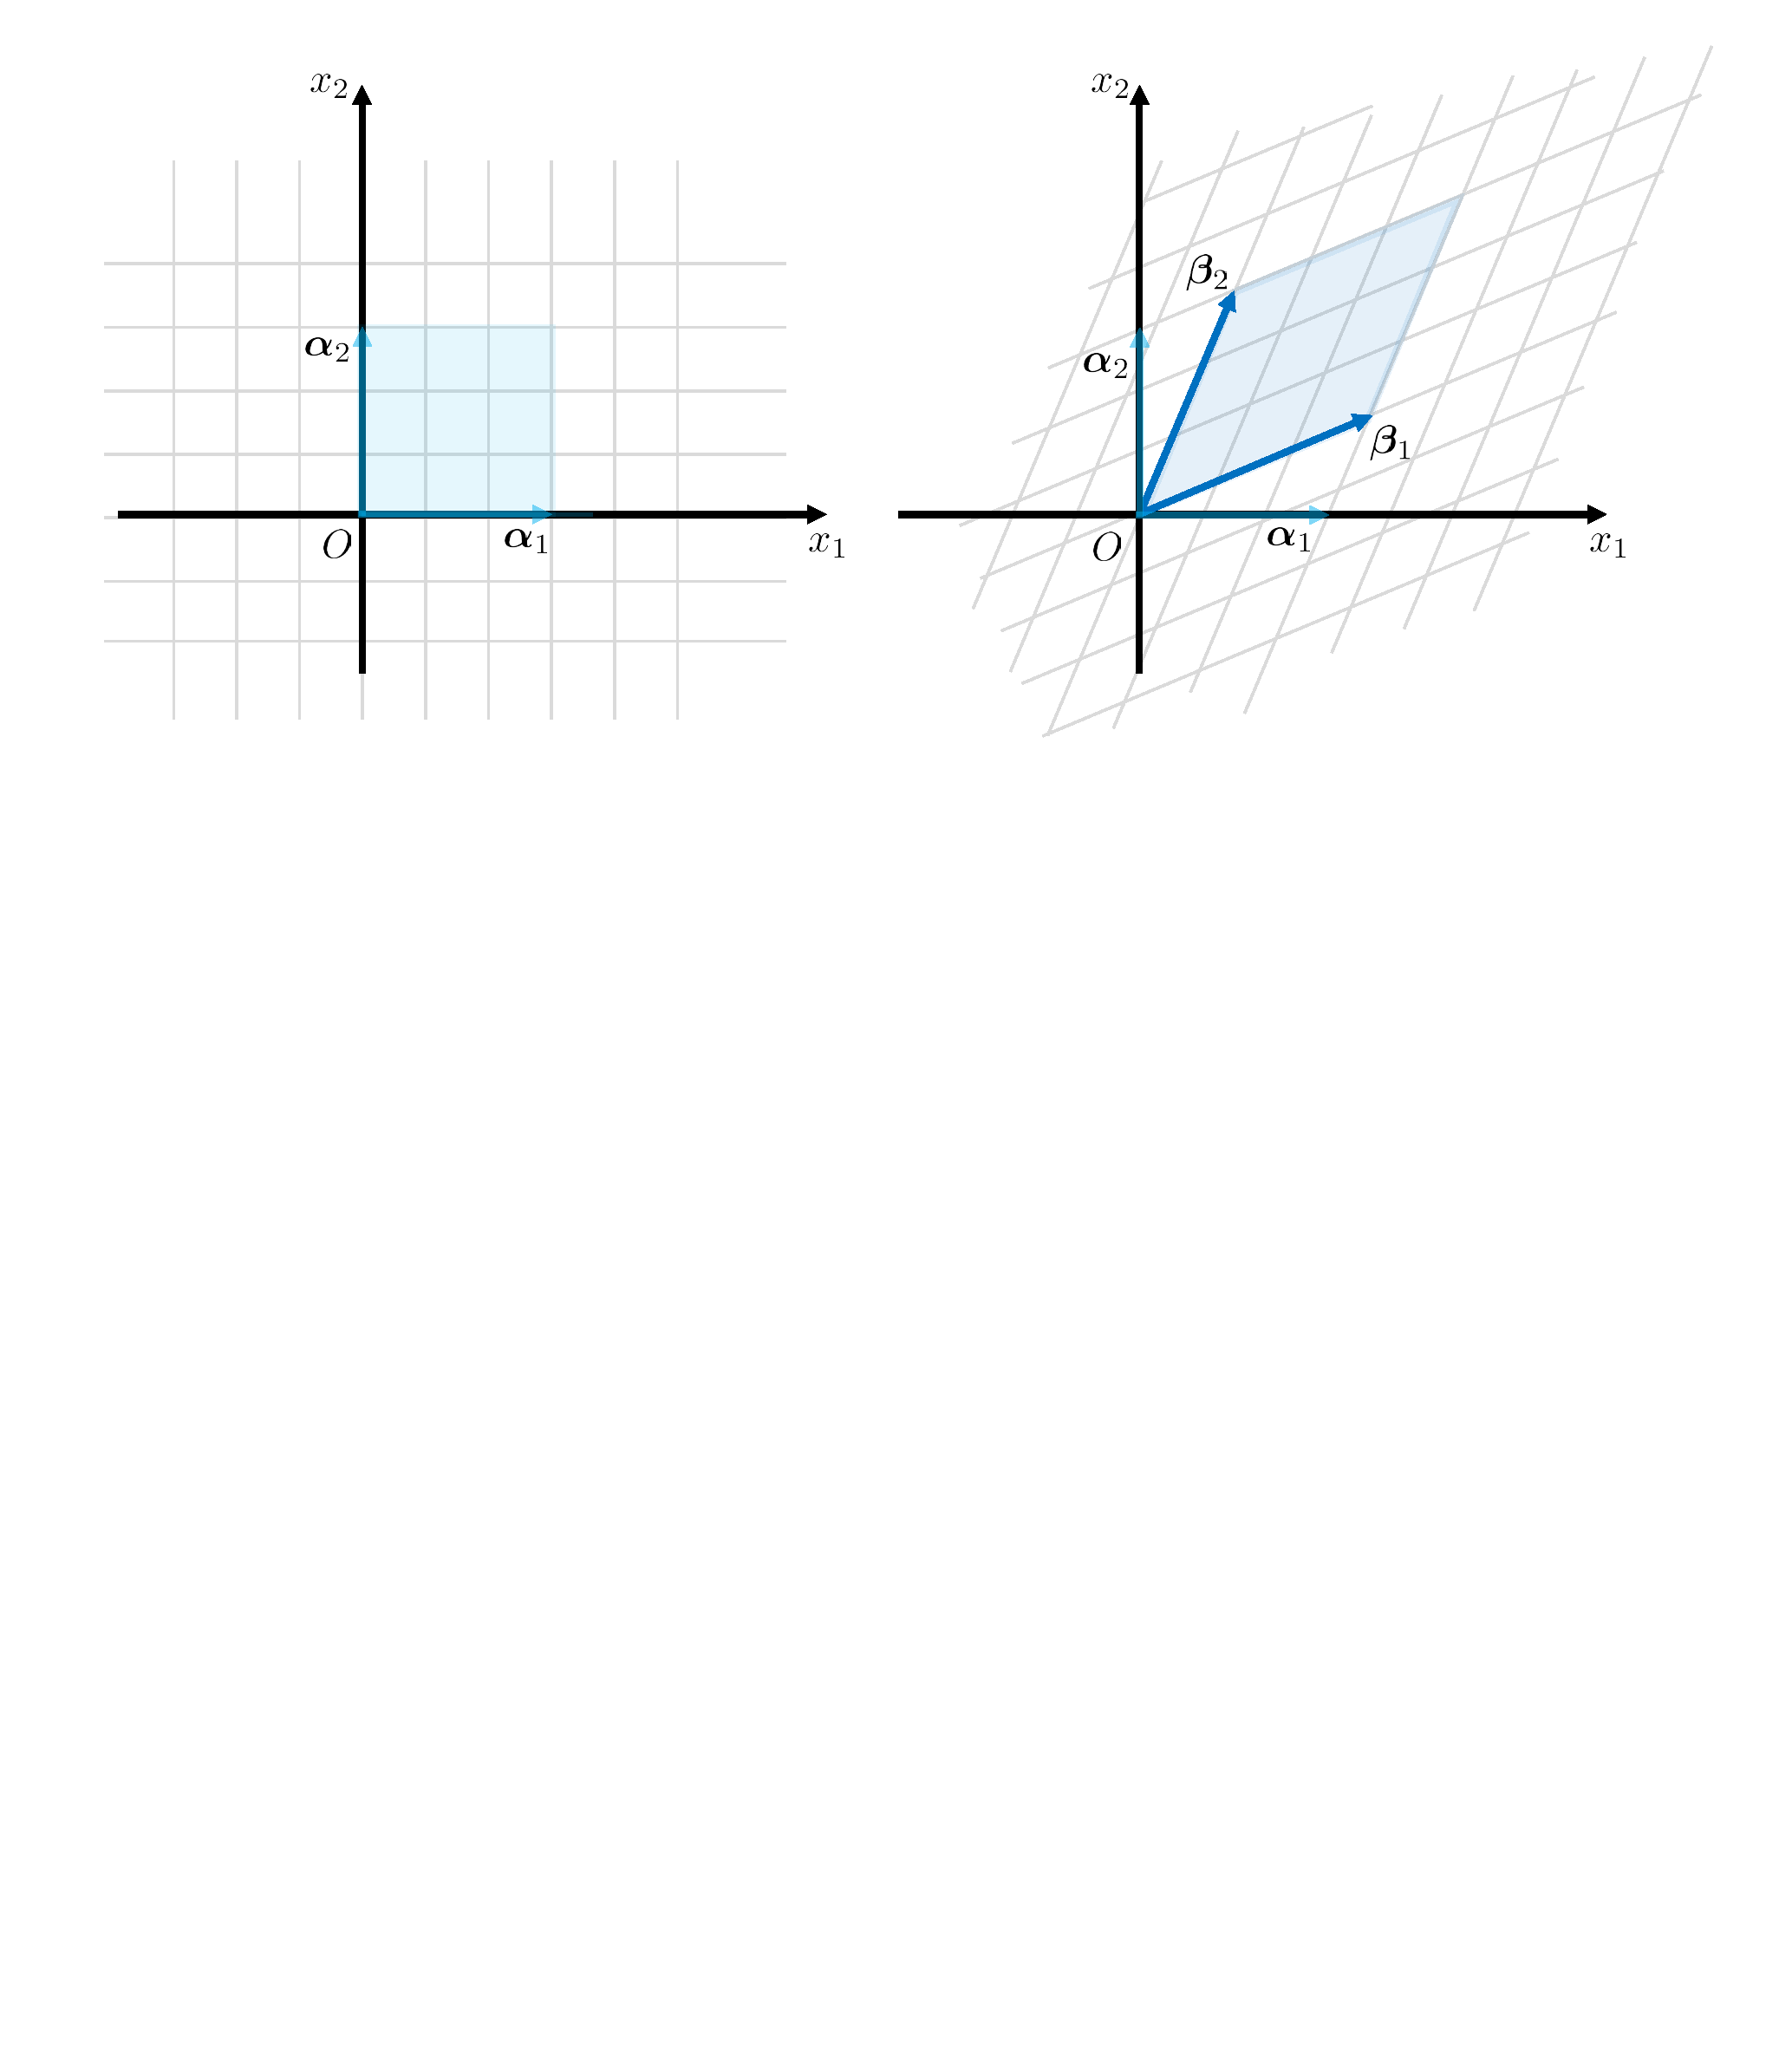
\includegraphics[trim=0 25cm 0 0, clip, width=1\textwidth]{fig_detarea.pdf}
    \caption{线性变换下的面积变化}
    \label{fig:detarea}
\end{figure}





以$\mathbb{R}^2$上5类基本的线性变换为例（图\ref{fig:area}）.
$\bm{\alpha}_1 = (1,0)$，
$\bm{\alpha}_2 = (0,1)$，
它们围出一个$1\times 1$的单位正方形，
面积为$1$.
它变换之后是由$\bm{\beta}_1,\bm{\beta}_2$围成的平行四边形，
面积已在图中标示出来.

其中，反射变换的结果是比较特殊的:
反射前后的图形如同左手和右手的区别，
虽然形状和大小都没有变化，
但是却不能通过平移和旋转使它们重合.
在图示的例子里，
无法通过$\mathbb{R}^2$内的平移和旋转使$\bm{\beta}_1,\bm{\beta}_2$
与$\bm{\alpha}_1,\bm{\alpha}_2$分别对应重合.
这种因“翻面”
而导致的方向性变化，
通过加一个负号来指示.
这种带正负号的面积称为\textbf{有向面积}.
在反射变换下，
单位正方形的有向面积变为$\bm{S} = -1$.

另外，
注意平行投影变换也是很特殊的.
因为它的效果是将单位正方形给“拍扁”了，
是一种降维打击，
有向面积变为$\bm{S} = 0$.
容易看出这是不可逆线性变换
（对应矩阵不满秩，
向量组线性相关）独有的性质.



\begin{figure}[H] 
    \centering
    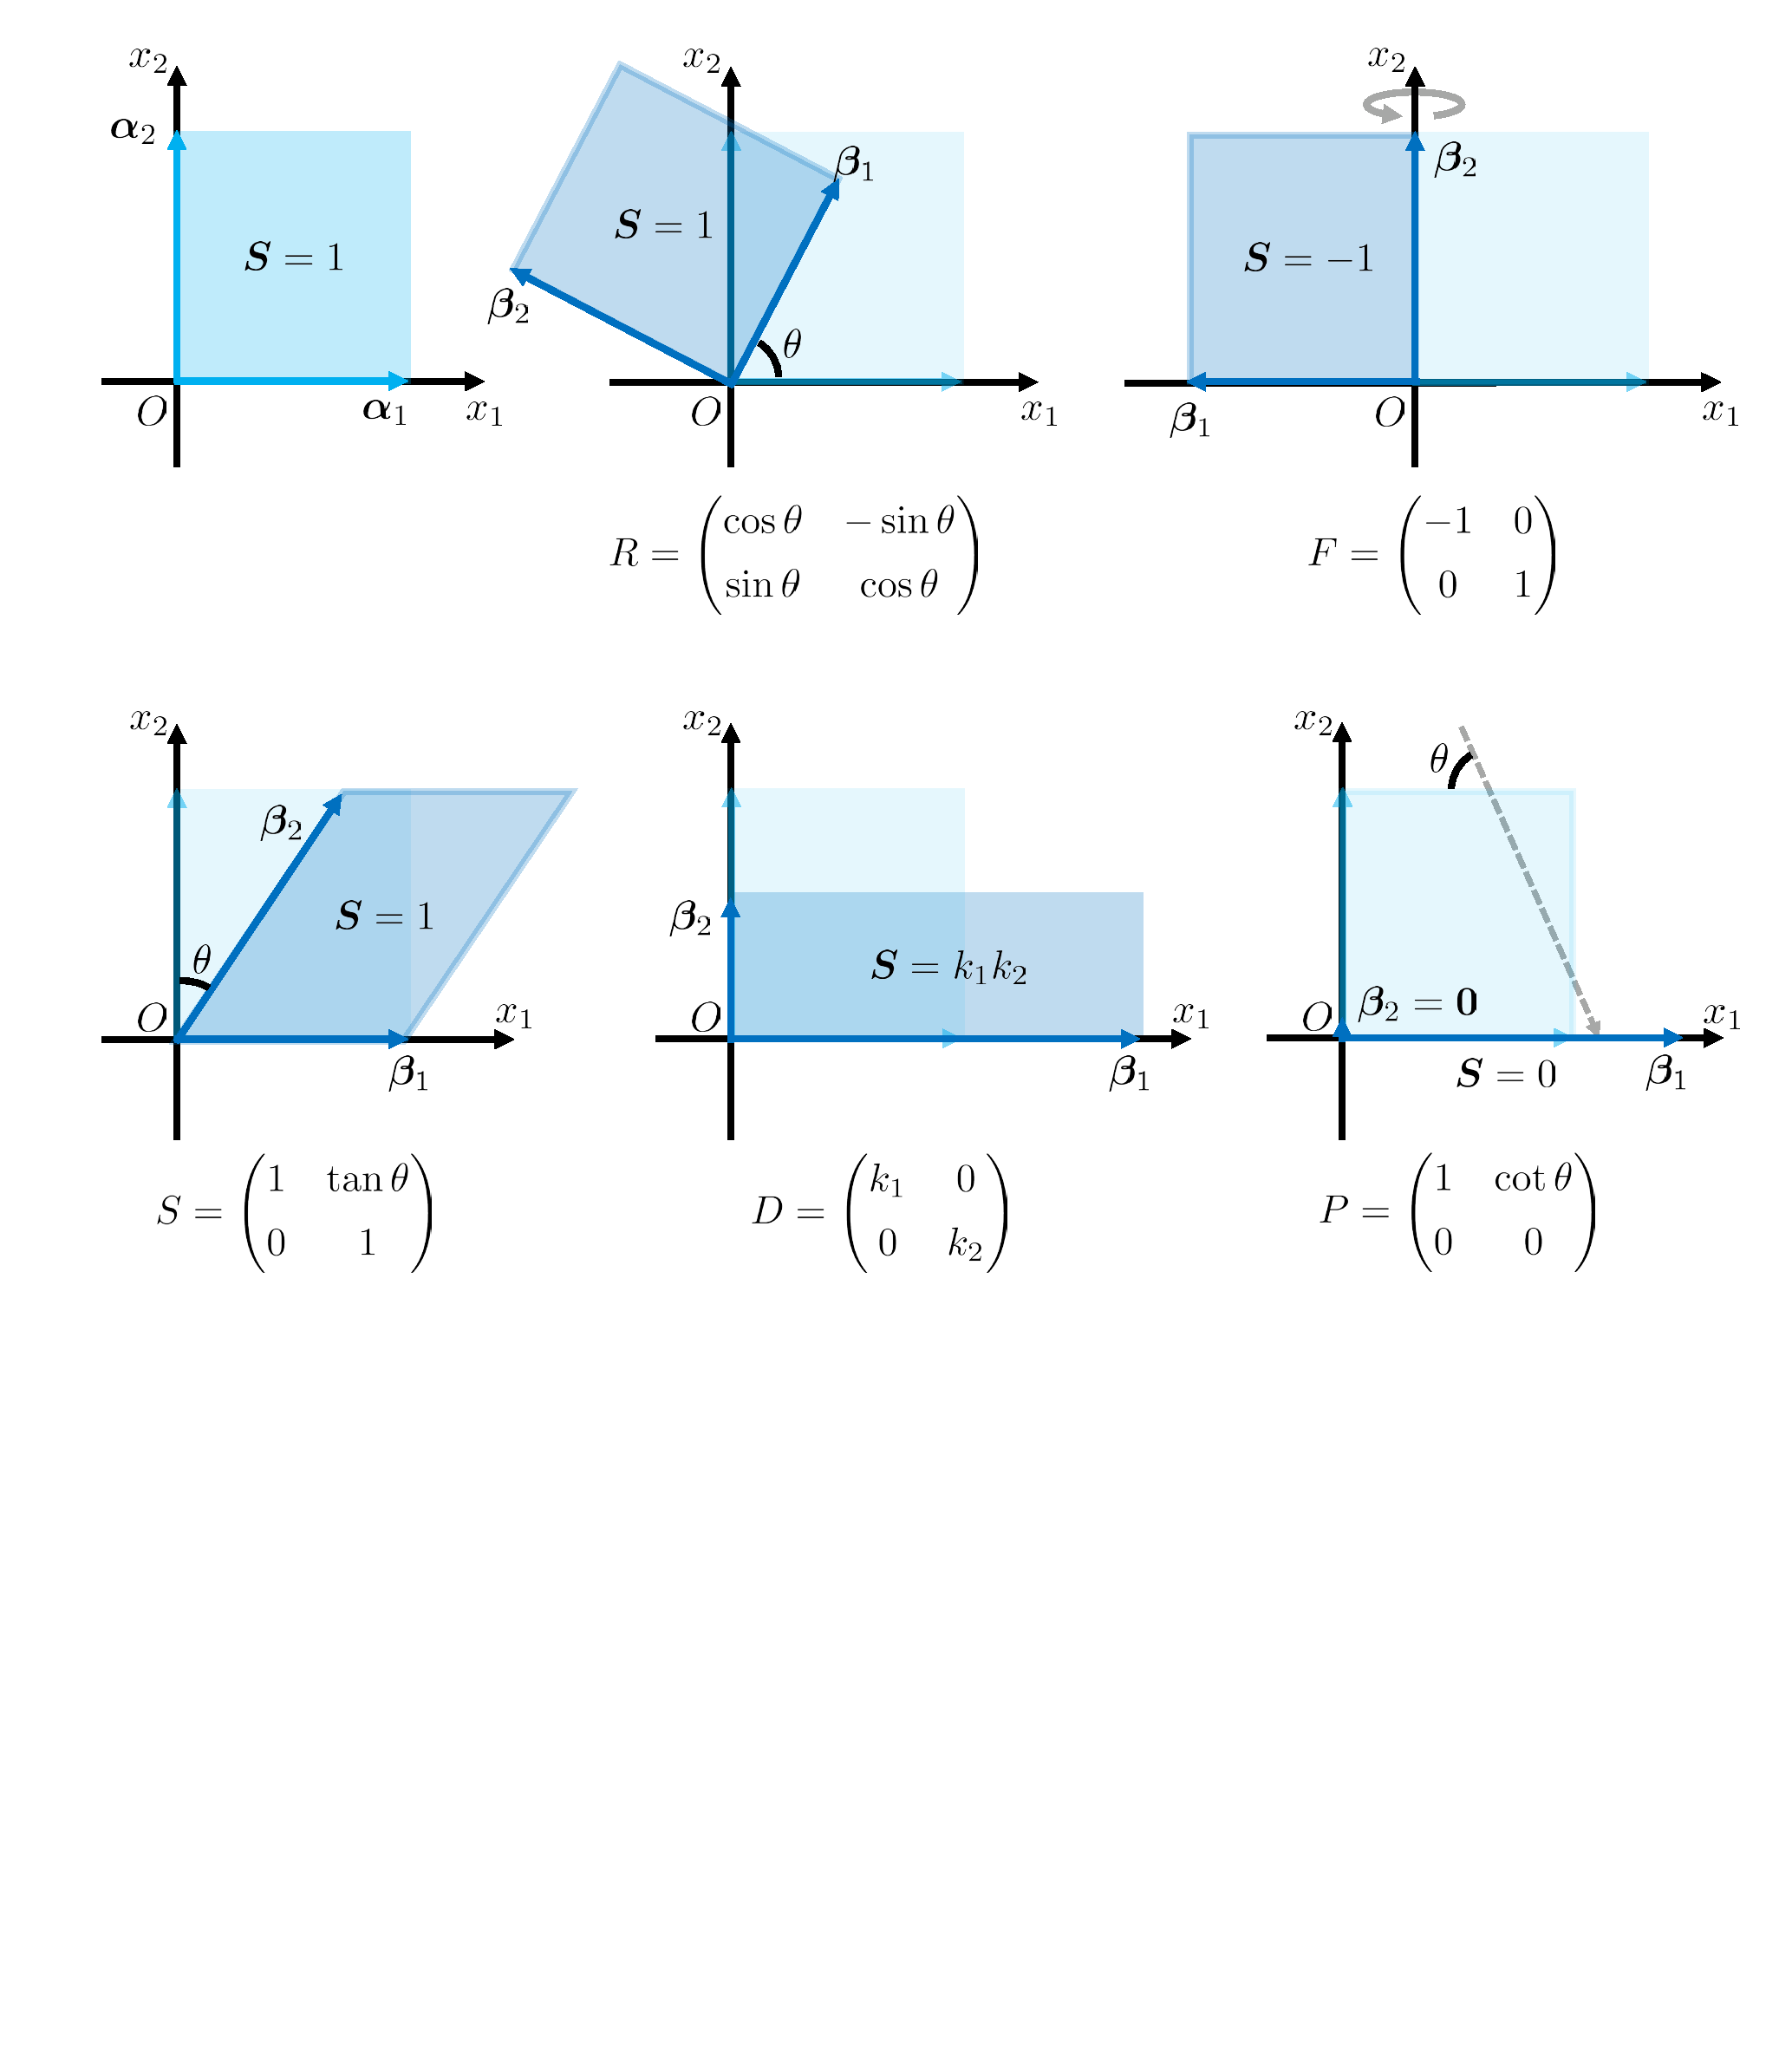
\includegraphics[trim=0 14cm 0 0, clip, width=1\textwidth]{fig_area.pdf}
    \caption{5类基本的线性变换引起的有向面积变化}
    \label{fig:area}
\end{figure}

在一般的$\mathbb{R}^n$上，
我们也可以做类似的讨论.
原先在$2$维情形中，
考察了一组标准正交基围成的单位正方形，
经历线性变换之后所变成的平行四边形（或者退化为$1$维的图形）的有向面积.
相应的，
在$3$维空间中，
我们考察单位立方体经变换后，
三个向量所围成的平行六面体的\textbf{有向体积}.
那么，
在$n$维空间中，
我们就需要考察$n$个向量所围出的
“$n$维平行方体”的“有向体积”.


\begin{figure}[H] 
    \centering
    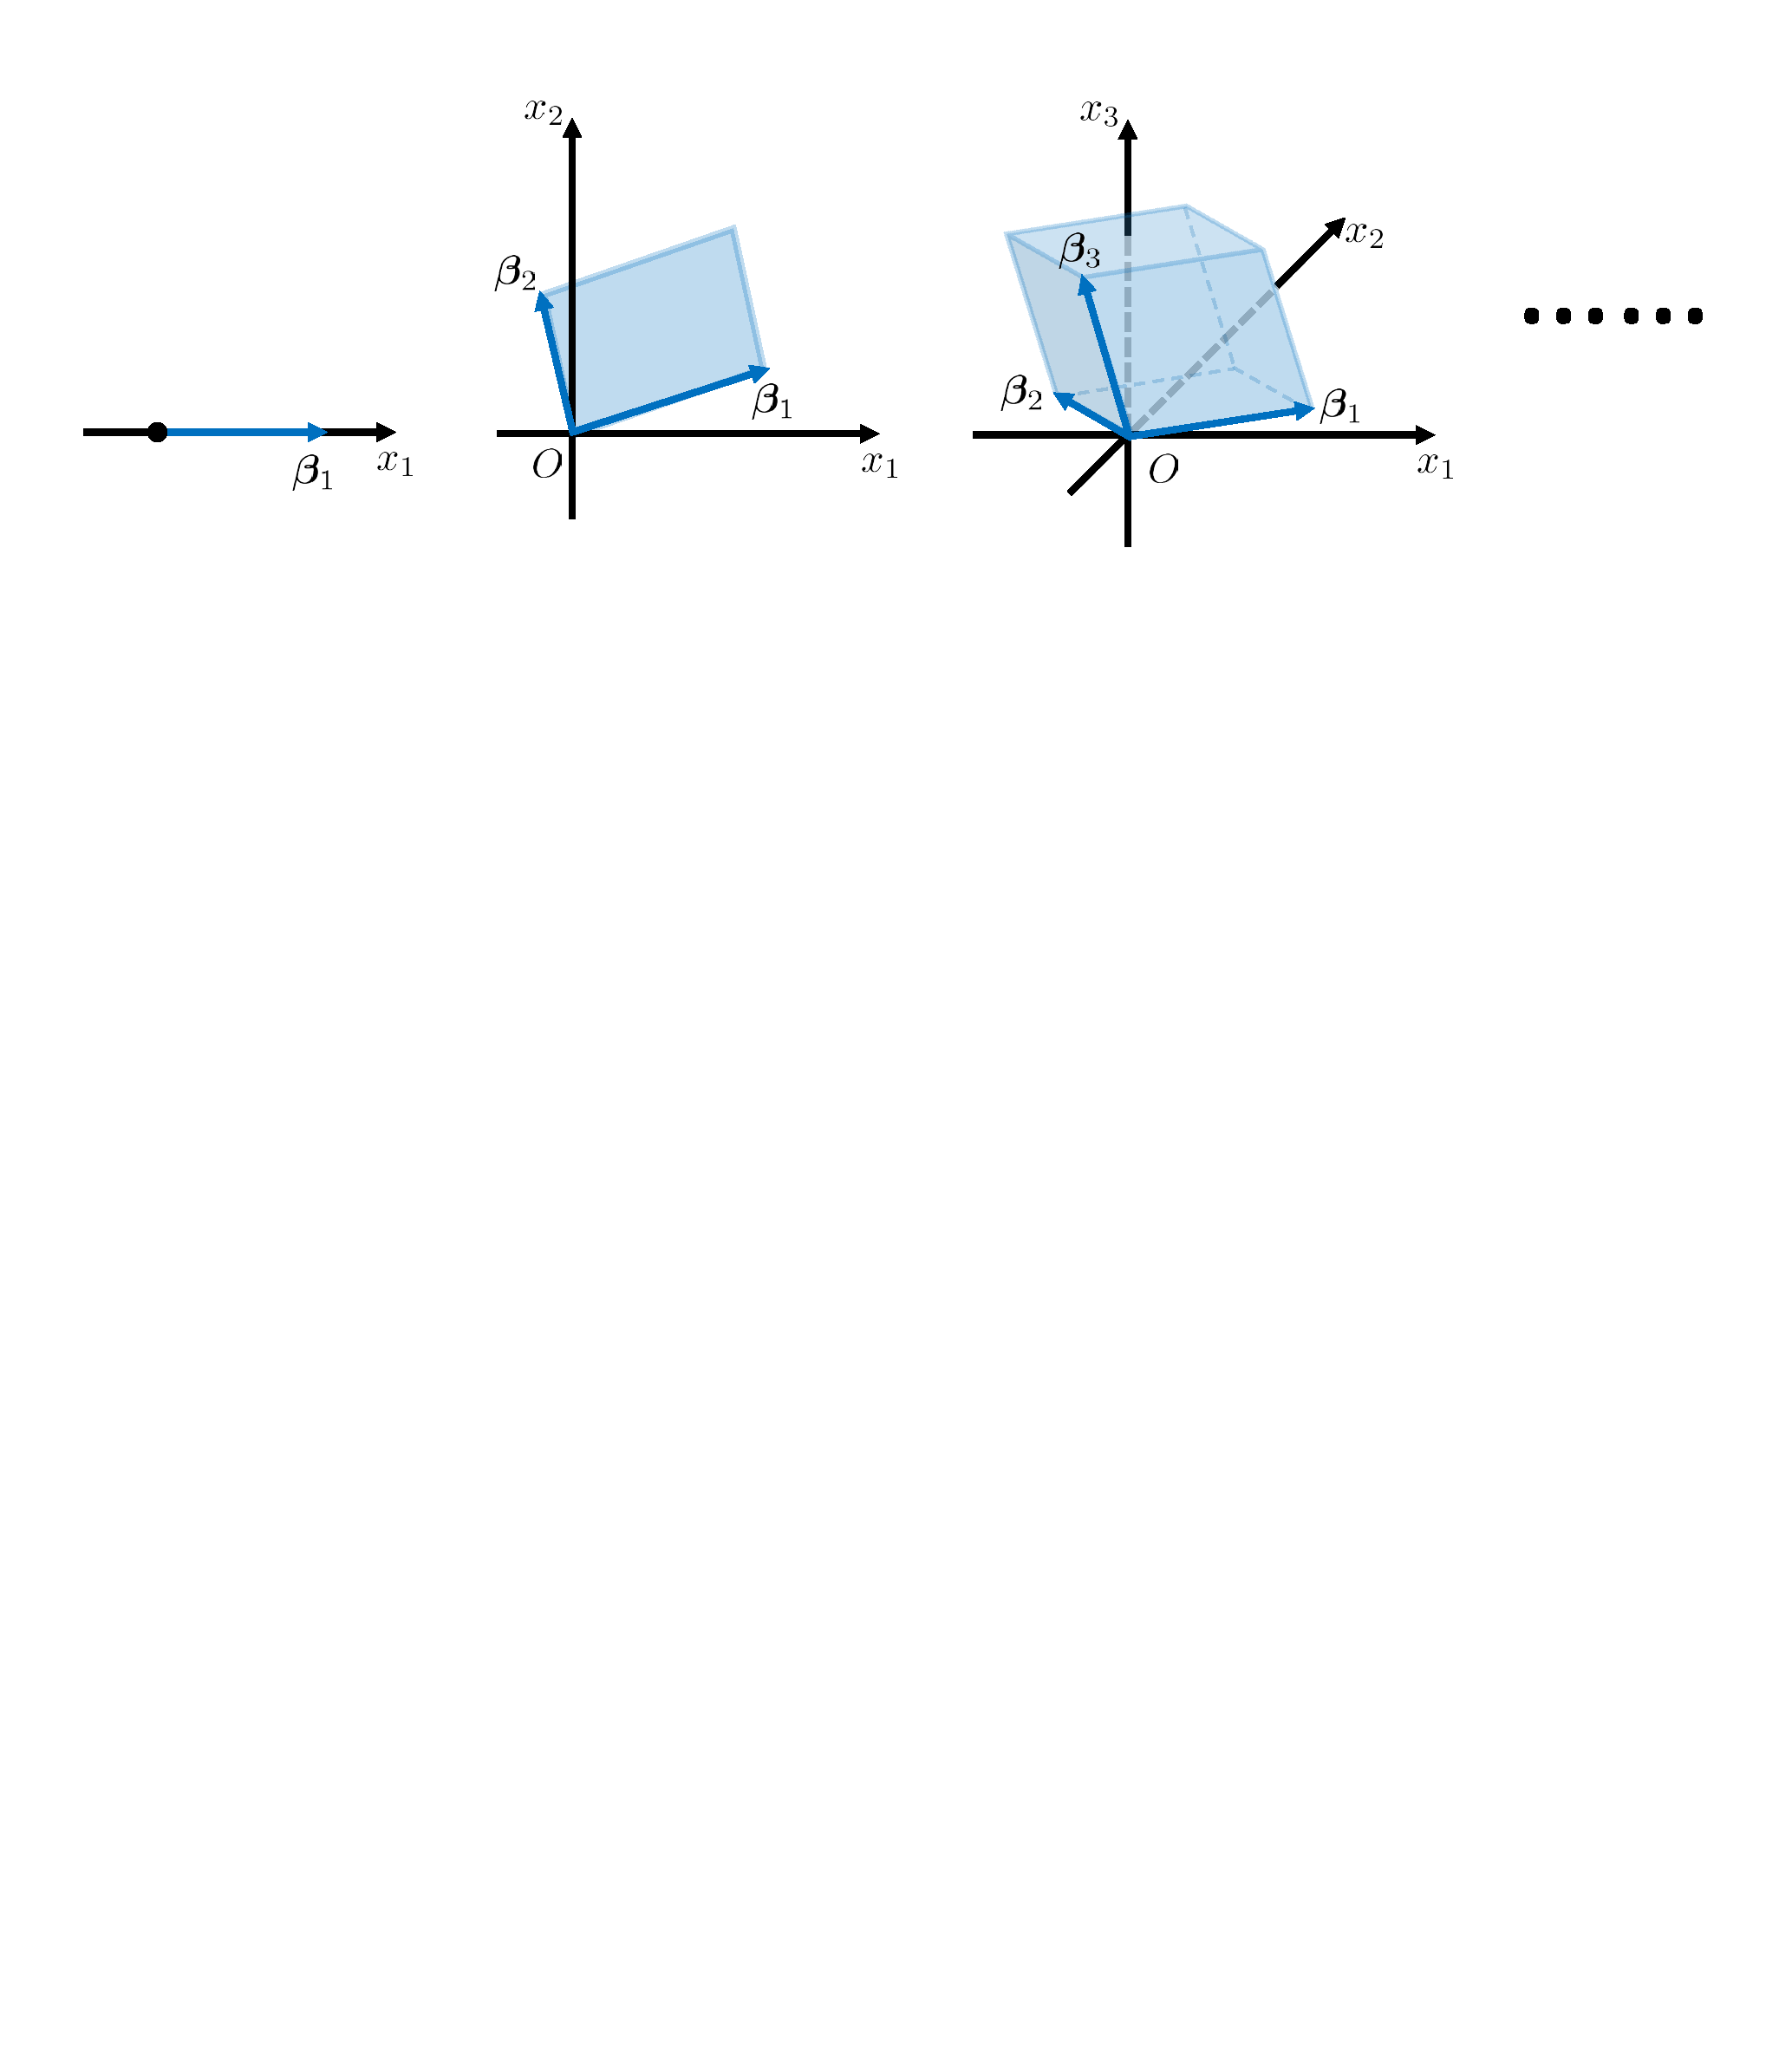
\includegraphics[trim=0 29cm 0 0, clip, width=1\textwidth]{fig_size.pdf}
    \caption{$n$维平行方体的$n$维有向体积}
    \label{fig:size}
\end{figure}

这就引出了行列式的一个几何定义：
对于一个$n$阶方阵
$A = (\bm{\beta}_1 , \bm{\beta}_2, \cdots , \bm{\beta}_n)$，
定义它的\textbf{行列式}
为$\bm{\beta}_1 , \bm{\beta}_2, \cdots , \bm{\beta}_n$
\textbf{所围出的$n$维平行方体的有向体积（有向长度、面积、体积……）}，
记作$\det A$或$\det (\bm{\beta}_1 , \bm{\beta}_2, \cdots , \bm{\beta}_n)$
或$|A|$.


这里，
$(\bm{\beta}_1 , \bm{\beta}_2, \cdots , \bm{\beta}_n)$表示以
$\bm{\beta}_1 , \bm{\beta}_2, \cdots , \bm{\beta}_n $为列向量组的矩阵.
根据矩阵乘法的规则，
容易验证$A \bm{e}_j = \bm{\beta}_j$，
其中$\bm{e}_j$是第$n$个标准正交基.
因此，
行列式的定义合乎我们开头讨论的背景：
它表示的是$n$维单位立方体经过线性变换之后，
得到的图形的有向体积；
这也恰是任何图形在线性变换下大小伸缩的比例.

当然，
这定义目前还不是十分严谨，
因为我们尚未说清楚什么是“$n$维的有向体积”.
我们只了解$1$维（有向长度）、
$2$维（有向面积）和
$3$维（有向体积）.
可以从低维情形中得到启示，
设置一些“有向体积”应当满足的标准，
并让这些标准唯一确定一个函数$\det$.
接下来就列出这些标准，
可以将其视为行列式的一个较严谨的定义.
\medskip

\textbf{定义（行列式的有向体积定义）}~~
\textit{对于$\bm{\beta}_1 , \bm{\beta}_2 , \cdots , \bm{\beta}_n \in \mathbb{K}^n$，
定义行列式是一个函数
$\det: (\bm{\beta}_1 , \bm{\beta}_2 , \cdots , \bm{\beta}_n) \mapsto \mathbb{K}$，
满足：}

\textit{(1)反对称性：
$\det (\cdots \bm{\beta}_i , \cdots , \bm{\beta}_j, \cdots) = - \det (\cdots \bm{\beta}_j , \cdots , \bm{\beta}_i, \cdots)$.
即：交换两个列向量的顺序，
行列式的值变号.}

\textit{(2)数乘性：设$k \in \mathbb{K}$，
$\det (\cdots k\bm{\beta}_i , \cdots) 
= k \cdot \det (\cdots \bm{\beta}_i , \cdots) $.
即$\det $对于任何位置的列向量的数乘是线性的.}

\textit{(3)可加性：设$\gamma \in \mathbb{K}^n$，
$\det (\cdots \bm{\beta}_i + \bm{\gamma} , \cdots) = 
\det (\cdots \bm{\beta}_i, \cdots) + \det (\cdots \bm{\gamma}, \cdots) $.
即$\det $对于任何位置的列向量的加法是线性的.}


\textit{(4)规范性：$\det (\bm{e}_1 , \bm{e}_2 , \cdots ,\bm{e}_n) = 1$，
即$n$维单位立方体的有向体积是$1$.}


\begin{figure}[H] 
    \centering
    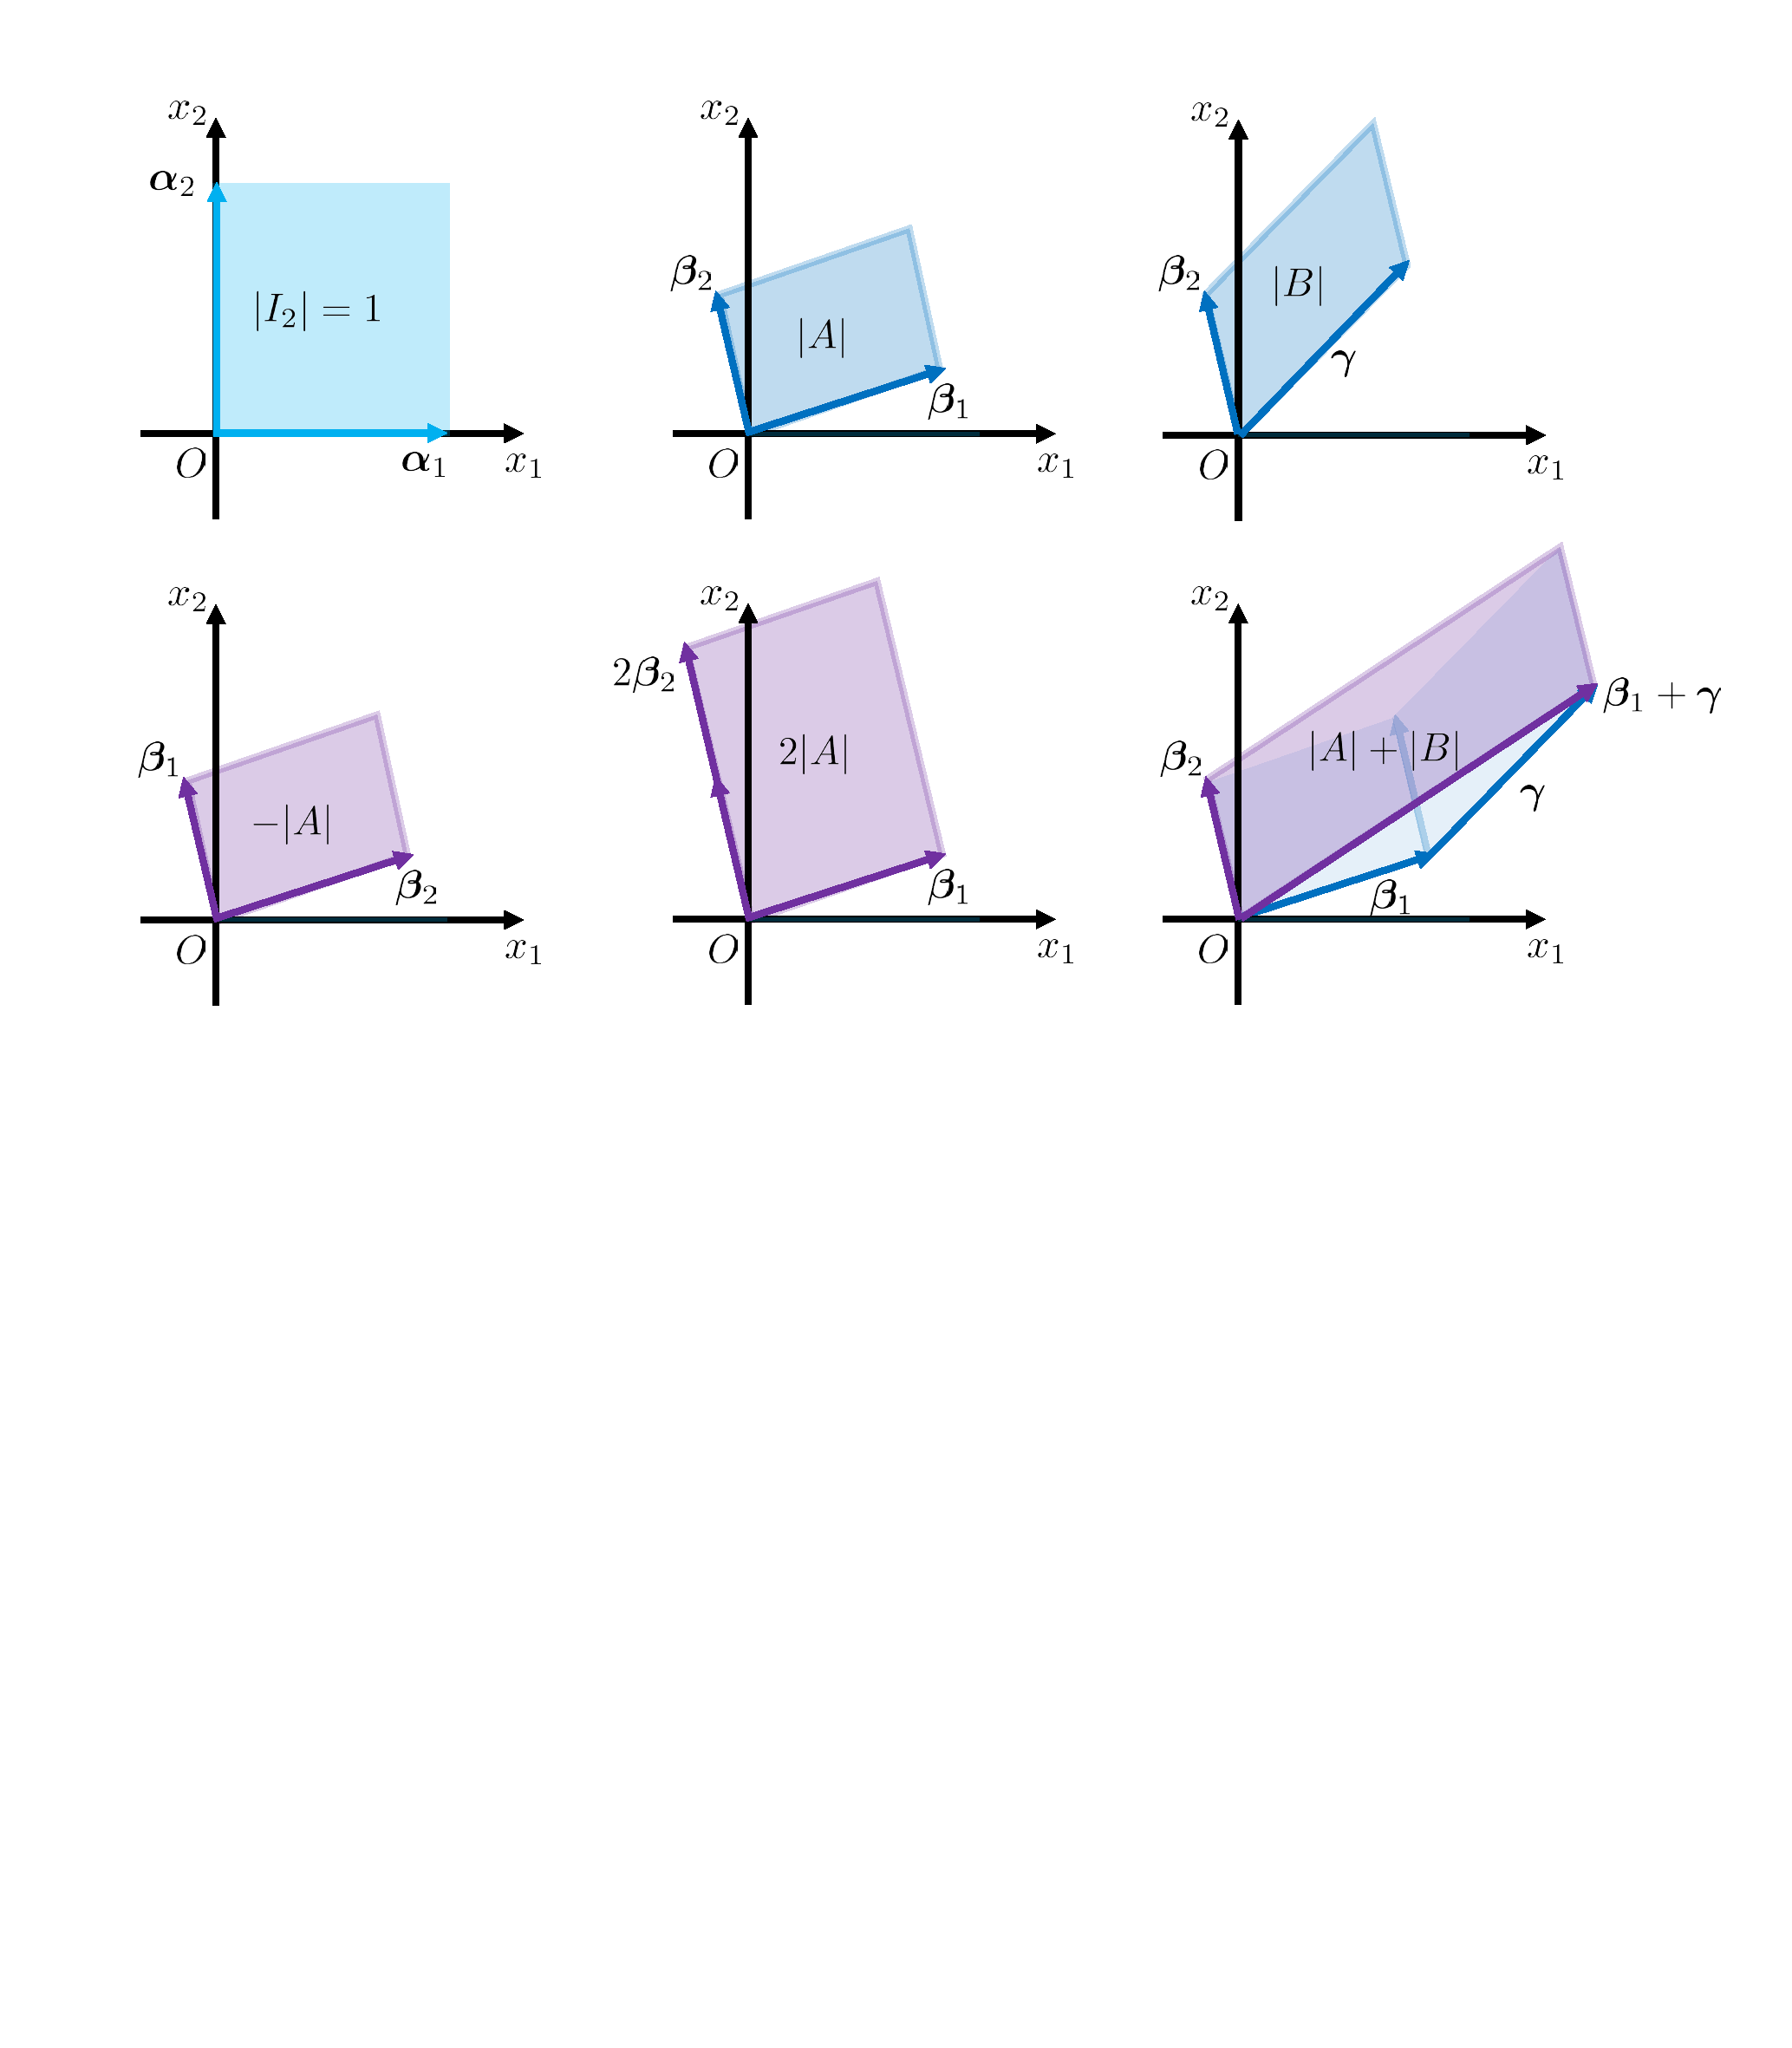
\includegraphics[trim=0 20cm 0 0, clip, width=1\textwidth]{fig_det.pdf}
    \caption{行列式的性质}
    \label{fig:det}
\end{figure}

可以从图
\ref{fig:det}
中看出设置其中部分规则的道理.
主要是数乘性和可加性（统称为线性性）：
平行四边形一条边长伸缩一定的比例，
其面积就伸缩相应的比例；
同底的两个平行四边形，
其另一边做向量加法得到的新的同底的平行四边形，
其面积是两个平行四边形之和.

现在我们自然要问：
有了这$4$条规则，
就已经唯一确定了$\det$的映射规则吗？
考察行列式的计算方法之后，
这一点就不言自明了.

\subsubsection{行列式的初等（列）变换算法}

本节我们考察如何直接从行列式的有向体积定义出发来计算行列式的值.
需要用到以下两个简单的命题：
\medskip

\textbf{命题3.1.1}~~
\textit{若矩阵有两个列向量相同，
则其行列式的值为$0$.
}

\textbf{证明\ }
根据反对称性，
交换那相同的两个列向量，
行列式应当变号.
但交换前后的矩阵是相同的，
行列式应当也相同.
因此行列式的值为$0$.
\qed

\medskip
\textbf{推论}~~
\textit{若矩阵有两个列向量共线，
则其行列式的值为$0$.}
\medskip


\textbf{命题3.1.2}~~
\textit{把矩阵的一个列向量$k$倍加到另一个列向量上，行列式的值不变.}

\textbf{证明\ } 
$\det (\cdots \bm{\beta}_i + k \bm{\beta}_j, \cdots , \bm{\beta}_j, \cdots) 
    = \det (\cdots \bm{\beta}_i, \cdots , \bm{\beta}_j, \cdots) +
    \det (\cdots k \bm{\beta}_j, \cdots , \bm{\beta}_j, \cdots) 
    = \det (\cdots \bm{\beta}_i, \cdots , \bm{\beta}_j, \cdots)$ \qed

\medskip

有了命题3.1.2，
再加上定义中的反对称性与数乘性，
我们就知道了行列式在初等列变换（交换两列、列的数乘、列的）
下的值如何变化.
因此，
我们只需要对矩阵进行初等列变换，
直至变成单位矩阵即可.
实际上计算的时候还可以更方便：
只需把一个方阵化为\textbf{上三角矩阵}或者\textbf{下三角矩阵}，
形如：

\begin{eq1}
    \begin{pmatrix}
        a_1 & * & * & \cdots & * \\[2pt]
        0 & a_2 & * & \cdots & * \\[2pt]
        0 & 0 & a_3 & \cdots & * \\[2pt]
        \vdots& \vdots & \vdots & \ddots & \vdots  \\[2pt]
        0 & 0 & 0 & \cdots & a_n 
    \end{pmatrix}
    ~~~~~~~~~~
    \begin{pmatrix}
        a_1 & 0 & 0 & \cdots & 0 \\[2pt]
        * & a_2 & 0 & \cdots & 0 \\[2pt]
        * & * & a_3 & \cdots & 0 \\[2pt]
        \vdots& \vdots & \vdots & \ddots & \vdots  \\[2pt]
        * & * & * & \cdots & a_n 
    \end{pmatrix}\\[12pt]
\end{eq1}

\textbf{上（下）三角矩阵的行列式的值是对角元的乘积，
即$a_1 a_2 \cdots a_n$}.
当对角元全都非零时，
这一点是很明了的，
因为很容易把上（下）三角矩阵通过初等列变换化成相应的\textbf{对角矩阵}，
而行列式的值不变.
对角线有零元的情况（此时行列式的值为$0$），
对目前而言证明起来有些复杂，
保留到后文中解决.

\subsection{行列式的展开算法}

\subsubsection{行列式的逆序数定义}

你可能注意到，
上一节中给出的行列式的有向体积定义与教科书中给出的定义完全不同.
后者涉及到排列和逆序数的概念，
与线性映射的关联不那么紧密.
但是提出这种定义的动机是容易理解的：
虽然有向体积定义自然地导出了行列式的初等变换算法，
可这毕竟只是一个计算的程序，
我们仍然希望能直接给出一个任意行列式的表达式.
我们来探究这个问题.

先考察最简单的$2$阶矩阵$A = (a_{ij}) = (\bm{\beta}_1,\bm{\beta}_2)$：

\begin{eq1}
    \det A 
    =
    \begin{vmatrix}
        a_{11} & a_{12}  \\[2pt]
        a_{21} & a_{22}  \\[2pt]
    \end{vmatrix}\\[12pt]
\end{eq1}

把每个列向量
展开为标准正交基的线性组合
$\bm{\beta}_i = a_{1i}\bm{e}_1 + a_{2i}\bm{e}_2~(i=1,2)$.
代入进行列式，
然后利用行列式的线性性质展开：

\begin{eq1}
    \det A 
    &= \det  (\bm{\beta}_1,\bm{\beta}_2) \\[4pt]
    &= \det  (a_{11}\bm{e}_1 + a_{21}\bm{e}_2 ~,~ 
    a_{12}\bm{e}_1 + a_{22}\bm{e}_2) \\[4pt]
    &= \det (a_{11}\bm{e}_1 , a_{12}\bm{e}_1) + 
    \det (a_{11}\bm{e}_1 , a_{22}\bm{e}_2) +
    \det (a_{21}\bm{e}_2 , a_{12}\bm{e}_1) +
    \det (a_{21}\bm{e}_2 , a_{22}\bm{e}_2) \\[4pt]
    &= a_{11} a_{12}\det (\bm{e}_1 , \bm{e}_1) + 
    a_{11}a_{22}\det (\bm{e}_1 , \bm{e}_2) +
    a_{21}a_{12}\det (\bm{e}_2 , \bm{e}_1) +
    a_{21}a_{22}\det (\bm{e}_2 , \bm{e}_2) \\[12pt]
\end{eq1}

展开过后虽然有$4$项，
但注意$\det (\bm{e}_1 , \bm{e}_1) = \det (\bm{e}_2 , \bm{e}_2) = 0$，
实际上有用的只有$2$项，
即$\det A = a_{11}a_{22}\det (\bm{e}_1 , \bm{e}_2) +
    a_{21}a_{12}\det (\bm{e}_2 , \bm{e}_1)$.
其中，$\det (\bm{e}_1 , \bm{e}_2)$是单位矩阵的行列式，
值为$1$；
而$\det (\bm{e}_2 , \bm{e}_1)$是单位矩阵交换两列后的行列式，
值为$-1$.
因此行列式的值为$a_{11}a_{22} - a_{12}a_{21}$.

对于$3$阶行列式：

\begin{eq1}
    \det A 
    &= \det  (\bm{\beta}_1,\bm{\beta}_2,\bm{\beta}_3 ) \\[4pt]
    &= \det  (a_{11}\bm{e}_1 + a_{21}\bm{e}_2 + a_{31}\bm{e}_3 ~,~ 
    a_{12}\bm{e}_1 + a_{22}\bm{e}_2 + a_{32}\bm{e}_3 ~,~
    a_{13}\bm{e}_1 + a_{23}\bm{e}_2 + a_{33}\bm{e}_3)\\[12pt]
\end{eq1}

从此例中可以领悟$n$阶行列式进行展开计算的一般方法.
利用行列式的线性性质完全展开之后，
应当有$n^n$个项，
但其中绝大多数项都是$0$.
有可能非零的项只可能是那些$\bm{e}_1,\bm{e}_2, \cdots , \bm{e}_n$在行列式中各出现一次的项，
共计$n!$个.
因此，
行列式的值可以表示为：

\begin{eq1}
    \det A =
    \sum_{i_1 i_2 \cdots i_n} a_{i_11}a_{i_22} \cdots a_{i_nn}\cdot \det (\bm{e}_{i_1},\bm{e}_{i_2} , \cdots ,\bm{e}_{i_n} )\\[12pt]
\end{eq1}

其中$i_1 i_2 \cdots i_n$是$1,2,\cdots,n$的任意一个排列.
我们只需要确定行列式
$\det (\bm{e}_{i_1},\bm{e}_{i_2} , \cdots ,\bm{e}_{i_n} )$
的值.
注意到它其实是单位矩阵的行列式$\det (\bm{e}_{1},\bm{e}_{2} , \cdots ,\bm{e}_{n} )$
调换向量顺序之后得到的，
而每次对换两个向量的顺序都会使得行列式变号.
我们只需要考察“进行多少次对换操作
能把一个任意排列$i_1i_2\cdots i_n$变成顺序排列$12\cdots n$”
——这个次数显然是不唯一的，
但真正重要的是它的奇偶性.
如果是偶数，
那么行列式的值为$1$；
如果是奇数，
那么行列式的值为$-1$.

一种标准的计算方法是计算一个排列的\textbf{逆序数}.
对于一个给定的排列$i_1i_2\cdots i_n$，
从中任取两个数，
如果大的数在前，
小的数在后，
那么称这一对数构成一个\textbf{逆序对}.
一个排列中逆序对的个数称为\textbf{逆序数}，
记作$\tau(i_1i_2\cdots i_n)$.
则行列式$\det (\bm{e}_{1},\bm{e}_{2} , \cdots ,\bm{e}_{n}) = (-1)^{\tau (i_1i_2\cdots i_n)}$.
有关排列的逆序数的算法的详细讨论参阅教科书.

行列式的展开式可以改写为：

\begin{eq1}
    \det A =
    \sum_{i_1 i_2 \cdots i_n} (-1)^{\tau(i_1 i_2 \cdots i_n)} a_{i_11}a_{i_22} \cdots a_{i_nn}\cdot \\[12pt]
\end{eq1}

这可以作为\textbf{行列式的逆序数定义}.

我们平时几乎不用逆序数定义来计算行列式，
因为计算量太大.
但是从这个定义中也能得到一些好处.
首先，
上（下）三角行列式是所有对角元的乘积，
这个命题从逆序数定义来看是比较显然的.
可以考察展开式每一项的构成：
除了正负符号以外，
每一项是矩阵中$n$个矩阵元的乘积，
且这些元素分居于$n$个不同的行，
和$n$个不同列中.
对于上（下）三角行列式，
展开式中唯一可能非零的项就是$n$个对角元组成的那一项，
其符号为正.

另外，
在展开式中，
默认每一项的列指标以顺序排列.
如果进一步把列指标打乱为一个任意的排列$j_1j_2\cdots j_n$，
则：

\begin{eq1}
    \det A =
    \sum_{i_1 i_2 \cdots i_n} (-1)^{\tau(i_1 i_2 \cdots i_n) + \tau(j_1 j_2 \cdots j_n)} 
    a_{i_1 j_1}a_{i_2 j_2} \cdots a_{i_n j_n}\\[12pt]
\end{eq1}

特别地，
取$i_1i_2\cdots i_n$是顺序排列$12\cdots n$.
则：

\begin{eq1}
    \det A =
    \sum_{i_1 i_2 \cdots i_n} (-1)^{\tau(j_1 j_2 \cdots j_n)} 
    a_{1 j_1}a_{2 j_2} \cdots a_{n j_n} \\[12pt]
\end{eq1}

注意这个展开式和原始的逆序数定义几乎一样，
只不过是把列换成了行.
这带给我们一条重要信息：
\textbf{行列式中的行与列关系是对等的}.
等价地有以下这条命题：
\medskip

\textbf{命题2.2.1}~~
\textit{矩阵转置不改变行列式的值}.

\medskip

由此我们知道，
3.1节中的所有（包括行列式的有向体积定义中）
关于列向量的表述，
换成行向量也是成立的.
用初等变换计算行列式的值时，
可以行变换和列变换并施.
这一点与计算矩阵的秩有异曲同工之妙.

\subsubsection{行列式按行（列）展开}

本小节给出一种比逆序数定义更温和一点的展开方式.
以$3$阶行列式为例.
根据线性性质，
可以按行列式的第一列进行拆分，
表示为三个行列式之和：

\begin{eq1}
    \begin{vmatrix}
        a_{11} & a_{12} & a_{13} \\[2pt]
        a_{21} & a_{22} & a_{23} \\[2pt]
        a_{31} & a_{32} & a_{33} 
    \end{vmatrix}
    &= 
    \begin{vmatrix}
        a_{11} & a_{12} & a_{13} \\[2pt]
        0 & a_{22} & a_{23} \\[2pt]
        0 & a_{32} & a_{33} 
    \end{vmatrix}
    +
    \begin{vmatrix}
        0 & a_{12} & a_{13} \\[2pt]
        a_{21} & a_{22} & a_{23} \\[2pt]
        0 & a_{32} & a_{33} 
    \end{vmatrix}
    +
    \begin{vmatrix}
        0 & a_{12} & a_{13} \\[2pt]
        0 & a_{22} & a_{23} \\[2pt]
        a_{31} & a_{32} & a_{33} 
    \end{vmatrix} \\[6pt]
    &=
    a_{11} 
    \begin{vmatrix}
        a_{22} & a_{23} \\[2pt]
        a_{32} & a_{33} 
    \end{vmatrix}
    +
    a_{21}
    \begin{vmatrix}
        a_{12} & a_{13} \\[2pt]
        a_{32} & a_{33} 
    \end{vmatrix}
    +
    a_{31}
    \begin{vmatrix}
        a_{12} & a_{13} \\[2pt]
        a_{22} & a_{23}
    \end{vmatrix} \\[12pt]
\end{eq1}

读者可自行验证第二个等号的正确性.
这个简单的例子启发我们，
对于一个$n$阶行列式，
可以按其中的某一列或某一行进行拆分，
表示成$n$个$n-1$阶行列式之和.
这样就实现了行列式的降阶.

为了叙述方便，
需要给出一个定义.
在$n$阶行列式$A$中任取一个元素$a_{ij}$，
将该元素所在的行和列划掉，
剩余的部分构成一个$n-1$阶行列式，
称为$a_{ij}$的\textbf{余子式}，
记为$M_{ij}$.
根据$a_{ij}$在矩阵中的位置，
为其余子式添加符号$(-1)^{i+j}$，
得到的结果称为$a_{ij}$的\textbf{代数余子式}，
记作$A_{ij} = (-1)^{i+j}M_{ij}$.
于是我们可以写出以下公式：
如果取$n$阶矩阵$A$的第$i$行进行拆分，
会得到：

\begin{eq1}
    \det A = \sum_{j=1}^{n} a_{ij} A_{ij}\\[12pt]
\end{eq1}

如果取第$j$列进行拆分，
会得到：

\begin{eq1}
    \det A = \sum_{i=1}^{n} a_{ij} A_{ij}\\[12pt]
\end{eq1}


也就是说，
\textbf{行列式的值等于其任意一行（列）的所有元素与其代数余子式乘积的和.}
这被称为行列式的\textbf{按行（列）展开.}
对此做两点注记：

\medskip

(1)~在一些书中会用按行（列）展开来作为行列式的递归定义，
因为该公式告诉我们如何用$n-1$阶行列式去计算$n$阶行列式，
而$1$阶行列式的值就是那唯一的元素本身.

\medskip

(2)~当行列式中有大量的元素为$0$时，
与逆序数展开相比，
按行（列）展开显然是一种更聪明的行列式算法.
选取$0$特别多的行（列）进行展开能为计算带来方便.
具体用法在习题部分讲解.

\clearpage

\subsubsection{行列式按$k$行（列）展开}

行列式的按行（列）展开可以进行推广.
在$n$阶矩阵$A$中，
任取其$k~(k < n)$个行（设取的是第$i_1,i_2,\cdots , i_k$行）
和$k$个列（设取的是第$j_1,j_2,\cdots , j_k$列），
它们交叉处的$k^2$个元素组成一个$k$阶行列式，
称为$A$的一个\textbf{$k$阶子式}，
记作：

\begin{eq1}
    A
    \begin{pmatrix}
        i_1 , i_2, \cdots , i_k  \\[2pt]
        j_1, j_2 , \cdots , j_k
    \end{pmatrix} \\[12pt]
\end{eq1}

从$A$中划去这$k$行$k$列，
剩余的元素拼成一个$n-k$阶行列式，
称为上述$k$阶子式的\textbf{余子式}.
在其前面乘上$(-1)^{p+q}$就成为上述$k$阶子式的\textbf{代数余子式}，
其中$p$和$q$分别为行指标和$p = i_1 + i_2 + \cdots + i_k$
与列指标和$q = j_1 + j_2 + \cdots + j_k$.
代数余子式记为：

\begin{eq1}
    \hat{A}
    \begin{pmatrix}
        i_1 , i_2, \cdots , i_k  \\[2pt]
        j_1, j_2 , \cdots , j_k
    \end{pmatrix} \\[12pt]
\end{eq1}

我们有如下的按$k$行（列）展开定理（Laplace定理）.

\medskip

\textbf{Laplace 定理} 
\textit{
设 \(A\) 是 \(n\) 阶矩阵，
在 \(A\) 中任取 \(k\) 行（列），
那么含于这 \(k\) 行（列）的全部 \(k\) 阶子式与其的代数余子式的乘积之和等于 \(\det A \).
即若取定 \(k\) 个行\(1 \leq i_1 < i_2 < \cdots < i_k \leq n\)，则：}

\begin{eq1}
    \det A = 
    \sum_{1 \leq j_1 < j_2 < \cdots < j_k \leq n} 
    A 
    \begin{pmatrix} i_1,i_2,\dots,i_k \\[2pt] 
        j_1,j_2,\dots,j_k 
    \end{pmatrix} 
    \hat{A} 
    \begin{pmatrix} i_1,i_2,\dots,i_k \\[2pt] 
        j_1,j_2,\dots,j_k 
    \end{pmatrix} \\[12pt]
\end{eq1}

\textit{同样若取定 \(k\) 个列\(1 \leq j_1 < j_2 < \cdots < j_k \leq n\)，
则：}

\begin{eq1}
    \det A = 
    \sum_{1 \leq i_1 < i_2 < \cdots < i_k \leq n}
     A 
     \begin{pmatrix} i_1,i_2,\dots,i_k \\[2pt]
         j_1,j_2,\dots,j_k 
    \end{pmatrix} 
    \hat{A} 
    \begin{pmatrix} i_1,i_2,\dots,i_k \\[2pt]
     j_1,j_2,\dots,j_k 
    \end{pmatrix}\\[12pt]
\end{eq1}

\medskip

一般来说，
直接用Laplace定理对行列式展开计算太复杂了.
但有一种情形很适用它.
考虑如下形状的行列式：


\begin{eq1}
    \begin{vmatrix}
    a_{11} & \cdots & a_{1k} & 0 & \cdots & 0 \\[2pt]
    \vdots & \ddots & \vdots & \vdots & \ddots & \vdots \\[2pt]
    a_{k1} & \cdots & a_{kk} & 0 & \cdots & 0 \\[2pt]
    a_{k+1,1} & \cdots & a_{k+1,k} & a_{k+1,k+1} & \cdots & a_{k+1,n} \\[2pt]
    \vdots & \ddots & \vdots & \vdots & \ddots & \vdots \\[2pt]
    a_{n1} & \cdots & a_{nk} & a_{n,k+1} & \cdots & a_{nn}
    \end{vmatrix}
    = 
    \begin{vmatrix}
        A & O \\[2pt]
        B & C
    \end{vmatrix} \\[12pt]
\end{eq1}

它可以看成是由$4$个矩阵拼在一起形成的大矩阵，
其中右上角的小矩阵块是零矩阵$O$.
根据Laplace定理容易算出：

\begin{eq1}
    \begin{vmatrix}
        A & O \\[2pt]
        B & C
    \end{vmatrix} 
    = |A| |C|
    \\[12pt]
\end{eq1}

更一般地，
考察如下形状的行列式：

\begin{eq1}
    \begin{vmatrix}
        A_1 & * & * & \cdots & * \\[2pt]
        O & A_2 & * & \cdots & * \\[2pt]
        O & O & A_3 & \cdots & * \\[2pt]
        \vdots & \vdots & \vdots & \ddots & \vdots \\[2pt]
        O & O & O & \cdots & A_n
    \end{vmatrix}
    ~~~~~~~
    \begin{vmatrix}
        A_1 & O & O & \cdots & O \\[2pt]
        * & A_2 & O & \cdots & O \\[2pt]
        * & * & A_3 & \cdots & O \\[2pt]
        \vdots & \vdots & \vdots & \ddots & \vdots \\[2pt]
        * & * & * & \cdots & A_n
    \end{vmatrix} \\[12pt]
\end{eq1}
其中每个位置都是一个矩阵块.
如果将矩阵块看成元素，
则以上两个行列式分别像上三角行列式和下三角行列式，
称为\textbf{分块上（下）三角行列式}.
计算它的行列式和计算上（下）三角行列式很类似：
\textbf{分块上（下）三角行列式等于所有对角矩阵块行列式的乘积}.
上面展示的两个行列式的值就是
$|A_1| |A_2| \cdots |A_n|$.

\subsection{与其他概念的联系}

\subsubsection{行列式与矩阵的秩}

计算行列式对于理解线性映射、矩阵和线性方程组有什么帮助？
有了第二章的铺垫，
实际上只要随便找一个切入点就能全部打通了.

我们在这里关注的要点是初等行（列）变换.
虽然对行列式做初等行（列）变换可能会改变它的值，
但注意到一个事实：
初等行（列）变换不会让非零的行列式变为零，
也不会让值为零的行列式变为非零.
矩阵的行列式为零和非零之间有什么无法逾越的差异吗？
根据第二章所学的矩阵等价（相抵）的思想，
我们一望相抵标准型便知答案：

\medskip

\textbf{命题3.3.1}~~
\textit{$n$阶方阵$A$的行列式非零，
当且仅当它相抵于$n$阶单位矩阵$I_n$.}

\textbf{证明\ }
$n$阶方阵$A$的行列式非零，
当且仅当它的相抵标准型的行列式非零，
而唯一一种行列式非零的$n \times n$相抵标准型就是$I_n$.
\qed 

\medskip

\textbf{推论1}~~
\textit{$n$阶方阵$A$的行列式非零，
当且仅当它满秩}.

\textbf{推论2}~~
\textit{$n$阶方阵$A$的行列式非零，
当且仅当它是可逆矩阵，
对应的线性映射是可逆映射}.

\textbf{推论3}~~
\textit{$n$阶方阵$A$的行列式非零，
当且仅当它的行（列）向量组线性无关，
从而是$\mathbb{K}^n$的一组基}.

\medskip

上述的推论只是对第$2$章的复习，
不再详细展开说明.
这里只强调一下“行列式非零”和“线性变换可逆”之间的联系.
如果一个线性映射的效果是把空间“压扁”，
那么它是不可逆的；
而“压扁”意味着任何图形经变换之后的有向体积都变为$0$.

\medskip

不满秩的方阵行列式都为零，
因此仅凭矩阵本身的行列式无法分辨它们秩的不同.
这里给出一个命题，
可以从行列式的角度确定一个矩阵的秩.

\medskip

\textbf{命题3.3.2}~~
\textit{一个矩阵的秩是其非零子式的最高阶数.}

\textbf{证明\ }
设$A_{m \times n}$的秩是$r$.
先证明$A$存在$r$阶非零子式：
取$A$的列向量组的一个极大线性无关组，
得到$A$的一个秩为$r$的$m \times r$子矩阵.
再取这个子矩阵的行向量组的一个极大线性无关组，
得到一个满秩的$r \times r$子矩阵，
其行列式非零.
这样就找到了$A$的一个$r$阶非零子式.

然后证明这就是最高阶的非零子式.
若$r<m$且$r<n$，
则$A$存在$k > r$阶子矩阵.
但子矩阵的秩至多是原矩阵的秩，
即$r$，
因此它不满秩，
行列式为$0$.
\qed

\medskip

在一些书中，
会将此作为矩阵的秩的定义.


\subsubsection{行列式与线性方程组}

尝试去解一个$2$个未知数，$2$条方程组的线性方程组$A\bm{x} = \bm{\beta}$.
其中系数矩阵$A = (\bm{\alpha}_1, \bm{\alpha}_2)$，
$\bm{x} = (x_1 , x_2)^{T}$，
$\bm{\beta} = (b_1 , b_2)^T$.
假定它有唯一解.
写出解的一般形式之后，
注意到表达式中的所有分子和分母均能写成$2$阶行列式的形式：

\begin{eq1}
    \begin{cases}
        b_1 = a_{11} \cdot x_1 + a_{12} \cdot x_2   \\[2pt]
        b_2 = a_{21} \cdot x_1 + a_{22} \cdot x_2
    \end{cases}
    \Longleftrightarrow ~~
    \begin{cases}
        x_1 =  \frac{a_{22}b_1 - a_{12}b_2}{a_{11}a_{22} - a_{12}a_{21}} = 
        \frac{\det (\bm{\beta} , \bm{\alpha}_2)}{\det (\bm{\alpha}_1 , \bm{\alpha}_2)}\\[12pt]
        x_2 = \frac{-a_{21}b_1 + a_{11}b_2}{a_{11}a_{22} - a_{12}a_{21}} = 
        \frac{\det (\bm{\alpha}_1 , \bm{\beta})}{\det (\bm{\alpha}_1 , \bm{\alpha}_2)}
    \end{cases}  \\[12pt]
\end{eq1} 

所有分母均为系数矩阵的行列式，
而$x_j$的分子是系数矩阵的第$j$列替换成常数列向量$\bm{\beta}$后的行列式.
这个规律是很好记忆的.
从表达式中还可以看出，
系数矩阵的行列式非零（分母非零）时，
方程组就有唯一解.
而如果系数矩阵的行列式为$0$，
且某一个$x_j$的分子行列式非零，
则形式上出现了$1/0$这样不合法的表达式，
说明此时方程组是无解的.
最后，如果所有分子和分母行列式都是$0$，
那么所有的解形式上都是$0/0$未定式，
它代表什么意思呢?
好像没法直接下定论.

综上所述，
对于系数矩阵是$n$阶方阵的线性方程组，
可以通过计算一些行列式来判定它解的情况，
并直接写出解的表达式.
这一系列判断和计算方法被称为\textbf{克拉默法则}.
教材上讲到克拉默法则时还没有讲矩阵的秩，
因此只能从简化行阶梯形矩阵的角度做出证明.
但是在这篇讲义里，
线性代数上半部分的内容已经接近尾声了，
我们应该可以把行列式、秩和线性方程组联系起来，
达成一个更好的理解.


\medskip

\textbf{定理（克拉默法则）}~~
\textit{设线性方程组$A\bm{x} = \bm{\beta}$中，
系数矩阵$A = (\bm{\alpha}_1 , \bm{\alpha}_2 , \cdots , \bm{\alpha}_n)$是$n$阶方阵.}
对于$j = 1,2,\cdots ,n$，
记矩阵$A_j = (\bm{\alpha}_1 , \cdots , \bm{\alpha}_{j-1} , \bm{\beta} , \bm{\alpha}_{j+1} , \cdots   \bm{\alpha}_n)$.

\smallskip

\textit{(1)~方程组有唯一解当且仅当$\det A \ne 0$，
此时$x_j = \frac{\det A_j}{\det A}$}.

\smallskip

\textit{(2)~当$\det A = 0$且存在某个$\det A_j \ne 0$时，方程组无解.}

\textit{(3)~当$\det A = \det A_j = 0$时，方程组可能有无穷多解，也可能无解.}

\smallskip

\textbf{证明\ }
回忆线性方程组解的判别准则（见2.2.1小节），
我们只需要研究两个问题.
第一，系数矩阵$A$是否列满秩？
第二，系数矩阵$A$与增广矩阵$\tilde{A}$的秩是否相等？

(1)~若$\det A \ne 0$，
即$\mathrm{rank}(A) = n$满秩.
而增广矩阵$\tilde{A} = (A , \bm{\beta})$
的秩至多为$n$，
因此$\mathrm{rank}(A) = \mathrm{rank}(\tilde{A}) = n$.
此时线性方程组有唯一解.
反之，
若线性方程组有唯一解，
直接得知$\mathrm{rank}(A) = n$.
至于解的表达式可直接通过计算验证成立，
这里省略.

(2)~若$\det A = 0$，
则$\mathrm{rank}(A) < n$不满秩.
此时若存在某个$\det A_j \ne 0$，
则$\mathrm{rank}(A_j) = n$满秩.
注意$A_j$可以看成$\tilde{A}$的一个$n$阶子矩阵
$(\bm{\alpha}_1 , \cdots , \bm{\alpha}_{j-1} , \bm{\alpha}_{j+1} , \cdots \bm{\alpha}_n, \bm{\beta}) $
的列向量重新排列之后得到的，
因此这个子矩阵和$A_j$同样是满秩，
行列式非零.
这就表明$\tilde{A}$有$n$阶非零子式，
而且没有更高阶的子式了.
所以$\mathrm{rank}(\tilde{A}) = n > \mathrm{rank}(A)$.
此时方程组无解.

(3)~若$\det A = \det A_j = 0$，
则$\mathrm{rank}(A) < n$，
因此方程组不可能是有唯一解的.
而$\tilde{A}$的所有$n$阶子式全为$0$，
因此$\mathrm{rank}(\tilde{A}) < n$.
不能确定$\mathrm{rank}(A)$与$\mathrm{rank}(\tilde{A})$的大小关系，
方程组可能是无解或者有无穷多解. \qed

\medskip

我们知道行列式有有向体积的几何意义.
对于克拉默法则所给出的解的表达式，
这里从几何角度给出一个解释.

以$2$阶的线性方程组$A \bm{x} = \bm{\beta}$为例.
$2$阶行列式代表的“有向体积”是平行四边形的有向面积.
图\ref{fig:crammer}左下展示了$\bm{\alpha}_1 , \bm{\alpha}_2, \bm{\beta}$三个向量，
求解线性方程组就是要为$\bm{\alpha}_1 , \bm{\alpha}_2$各确定一个系数$x_1,x_2$，
从而让它们线性组合出$\bm{\beta}$（右上）.
以求解$x_1$为例，
它可以理解为$\bm{\alpha}_1$需要伸缩的比例.
在图像上，
可以从$\bm{\beta}$的终点出发，作出$\bm{\alpha}_2$的平行线来确定出$x_1 \bm{\alpha}_1$（右下）.
不难看出，
$x_1 \bm{\alpha}_1$与$\bm{\alpha}_1$的长度之比，
恰是紫色平行四边形与蓝色平行四边形的面积之比，
用行列式表示出它们的面积，
就得到了克拉默法则中的表达式.
$x_2$的求解同理（左上）.



\begin{figure}[H] 
    \centering
    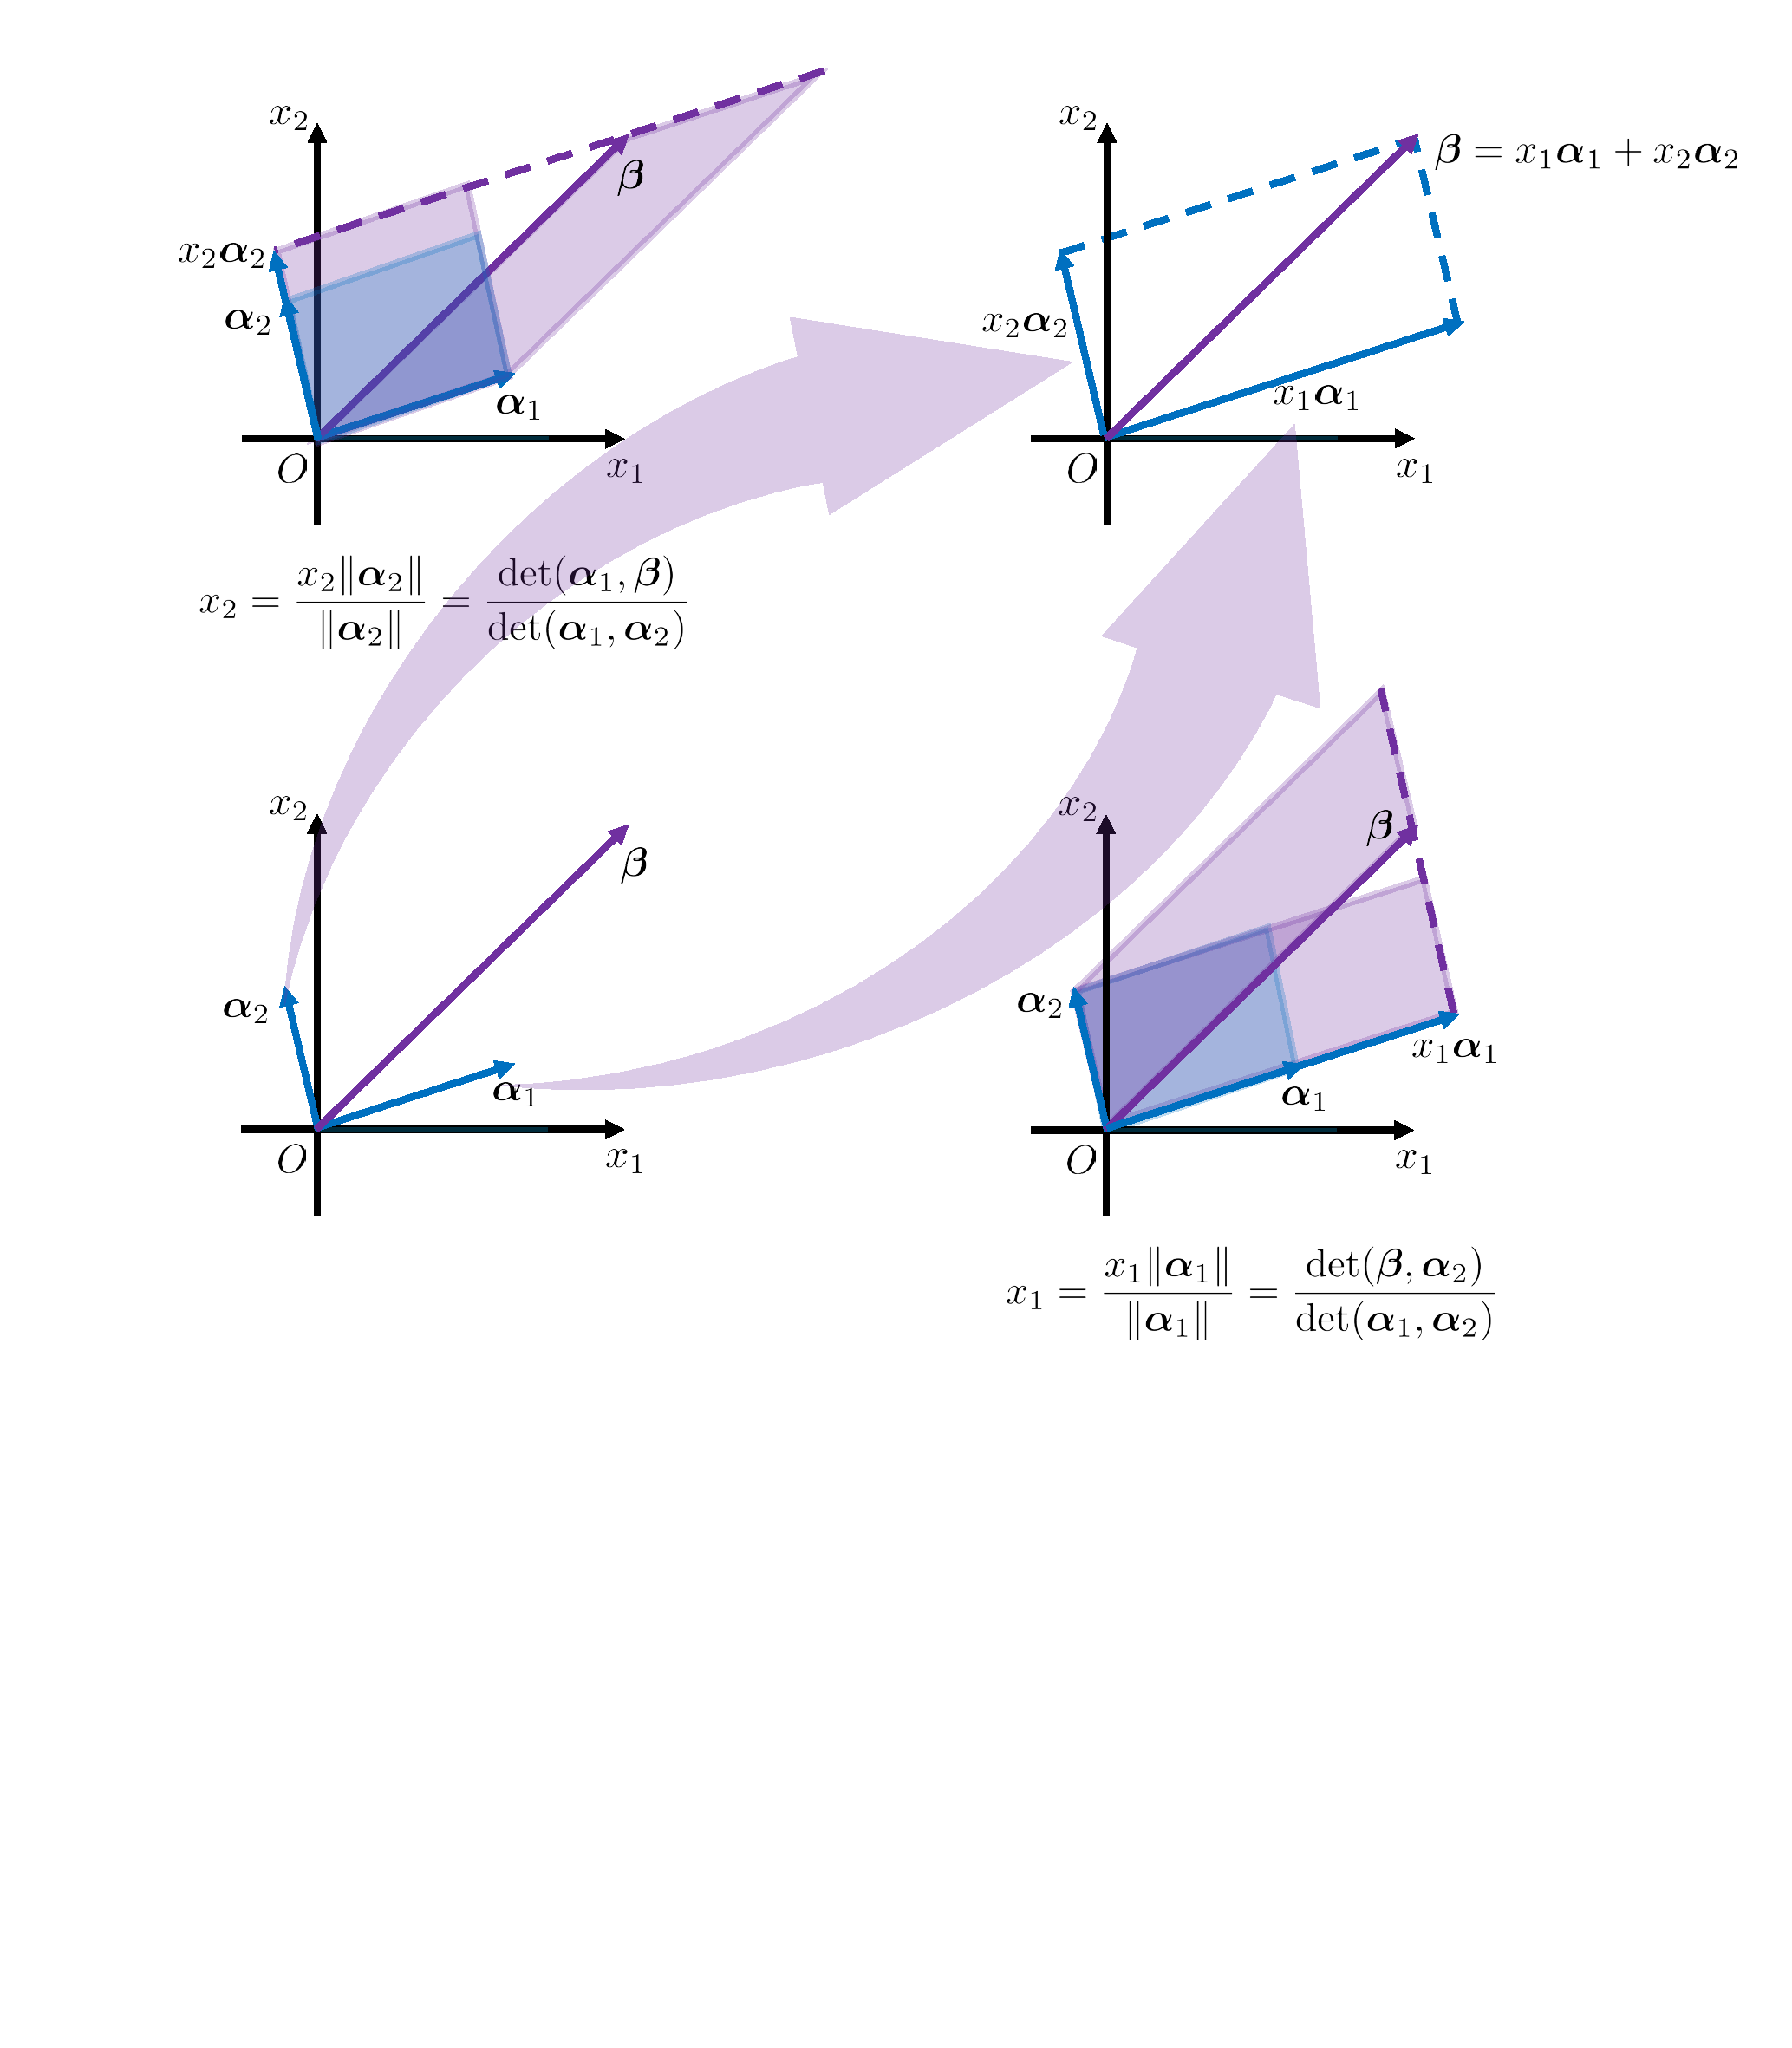
\includegraphics[trim=0 13cm 0 0, clip, width=1\textwidth]{fig_crammer.pdf}
    \caption{克拉默法则示意图}
    \label{fig:crammer}
\end{figure}


\subsection{习题}



\begin{example}
    计算行列式：【答案：$76$】
    \begin{eq1}
    \begin{vmatrix}
        1 & ~ & -2 & -2 & ~ \\[2pt]
        ~ & 1 & ~ & -2 & -2 \\[2pt]
        3 & ~ & -2 & ~ & ~ \\[2pt]
        ~ & 3 & ~ & -2 & ~ \\[2pt]
        ~ & ~ & 3 & ~ & -2
    \end{vmatrix}
    \end{eq1}
\end{example}

~\par

\begin{example}
    计算行列式：【答案：$(a_1 d_1 - b_1 c_1)(a_2 d_2 - b_2 c_2)$】
    \begin{eq1}
    \begin{vmatrix}
        a_1 & ~ & b_1 & ~  \\[2pt]
        ~ & a_2 & ~ & b_2  \\[2pt]
        c_1 & ~ & d_1 &  \\[2pt]
        ~ & c_2 & ~ & d_2 \\[2pt]
    \end{vmatrix}
    \end{eq1}
\end{example}
\begin{remark}
    化为分块对角行列式.
\end{remark}

~\par

\begin{example}
    计算$n$阶“鸡爪形”行列式：【答案：$a_1 - a_2 b_2 - \cdots - a_n b_n$】
    \begin{eq1}
    \begin{vmatrix}
        a_1 & a_2 & a_3 & \cdots & a_n \\[2pt]
        b_2 & 1 & 0 & \cdots & 0 \\[2pt]
        b_3 & 0 & 1 & \cdots & 0 \\[2pt]
        \vdots & \vdots & \vdots & \ddots & \vdots \\[2pt]
        b_n & 0 & 0 & \cdots & 1
    \end{vmatrix}
    \end{eq1}
\end{example}

\begin{remark}
    化为上（下）三角行列式.
\end{remark}

~\par

\begin{example}
    计算行列式：
    \begin{eq1}
    \begin{vmatrix}
        1 & 2 & 2 & 2 & 2 \\[2pt]
        2 & 2 & 2 & 2 & 2 \\[2pt]
        2 & 2 & 3 & 2 & 2 \\[2pt]
        2 & 2 & 2 & 4 & 2 \\[2pt]
        2 & 2 & 2 & 2 & 5
    \end{vmatrix}\\[12pt]
    \end{eq1}
\end{example}

\begin{remark}
    行列式中的$2$很多，
    利用全为$2$的第$2$列去把大量的$2$都消成$0$.
\end{remark}

\bigskip

\begin{example}
    计算行列式：
    \begin{eq1}
    \begin{vmatrix}
        2+a & 2 & 2 & 2 & 2 \\[2pt]
        2 & 2+b & 2 & 2 & 2 \\[2pt]
        2 & 2 & 2+c & 2 & 2 \\[2pt]
        2 & 2 & 2 & 2+d & 2 \\[2pt]
        2 & 2 & 2 & 2 & 2+e
    \end{vmatrix}
    \end{eq1}
\end{example}

~\par

\begin{example}
    计算行列式：【答案：$(-1)^{n-1} (n-1)2^{n-2}$】
    \begin{eq1}
        D_n = 
    \begin{vmatrix}
        0 & 1 & 2 & \cdots & n-2 & n-1 \\[2pt]
        1 & 0 & 1 & \cdots  & n-3 & n-2 \\[2pt]
        2 & 1 & 0 & \cdots & n-4 & n-3 \\[2pt]
        \vdots & \vdots & \vdots & \ddots & \vdots &\vdots \\[2pt]
        n-2 & n-3 & n-4 & \cdots & 0 & 1 \\[2pt]
        n-1 & n-2 & n-3 & \cdots  & 1 & 0 
    \end{vmatrix}
    \end{eq1}
\end{example}

~\par

\begin{example}
    计算$n$阶行列式【答案：斐波那契数列】：
    \begin{eq1}
        D_n =  
    \begin{vmatrix}
        1 & 1 & 0 & \cdots & 0 & 0 \\[2pt]
        -1 & 1 & 1 & \cdots  & 0 & 0 \\[2pt]
        0 & -1 & 1 & \cdots & 0 & 0 \\[2pt]
        \vdots & \vdots & \vdots & \ddots & \vdots &\vdots \\[2pt]
        0 & 0 & 0 & \cdots & 1 & 1 \\[2pt]
        0 & 0 & 0 & \cdots  & -1 & 1 
    \end{vmatrix}
    \end{eq1}
\end{example}

~\par


\begin{example}
    证明$n$阶行列式：
    \begin{eq1}
        D_n = 
    \begin{vmatrix}
        \cos \alpha & 1 & 0 & \cdots & 0 & 0 \\[2pt]
        1 & 2\cos \alpha & 1 & \cdots  & 0 & 0 \\[2pt]
        0 & 1 & 2\cos \alpha & \cdots & 0 & 0 \\[2pt]
        \vdots & \vdots & \vdots & \ddots & \vdots &\vdots \\[2pt]
        0 & 0 & 0 & \cdots & 2\cos \alpha & 1 \\[2pt]
        0 & 0 & 0 & \cdots  & 1 & 2\cos \alpha 
    \end{vmatrix}_{n}
    = \cos n \alpha
    \end{eq1}
\end{example}

~\par

\begin{example}
    证明$n$阶范德蒙德行列式：
    \begin{eq1}
        D_n = 
    \begin{vmatrix}
        1 & 1 & 1 & \cdots  & 1 \\[2pt]
        a_1 & a_2 & a_3 & \cdots  & a_n \\[2pt]
        a_1^2 & a_2^2 & a_3^2 & \cdots  & a_n^2 \\[2pt]
        \vdots & \vdots & \vdots & ~ & \vdots  \\[2pt]
        a_1^{n-2} & a_2^{n-2} & a_3^{n-2} & \cdots  & a_n^{n-2} \\[2pt]
        a_1^{n-1} & a_2^{n-1} & a_3^{n-1} & \cdots  & a_n^{n-1} \\[2pt]
    \end{vmatrix}_{n}
    = \prod_{1 \le j < i \le n} (a_i  - a_j)
    \end{eq1}
\end{example}

~\par

\begin{example}
    计算行列式：【答案：$8 \prod_{1 \le j < i \le 4} (\cos \theta _1 - \cos \theta _ j)$】
    \begin{eq1}
        D_n = 
    \begin{vmatrix}
        1 & \cos \theta_1 & \cos 2 \theta_1 & \cos 3 \theta_1 \\[2pt]
        1 & \cos \theta_2 & \cos 2 \theta_2 & \cos 3 \theta_2  \\[2pt]
        1 & \cos \theta_3 & \cos 2 \theta_3 & \cos 3 \theta_3  \\[2pt]
        1 & \cos \theta_4 & \cos 2 \theta_4 & \cos 3 \theta_4
    \end{vmatrix}
    \end{eq1}
\end{example}


\begin{example}
    计算$n$阶行列式：【答案：$\sum_{k=1}^{n}a_k \prod_{1 \le j < i \le n} (a_i - a_j)$】
    \begin{eq1}
        D_n = 
    \begin{vmatrix}
        1 & 1 & 1 & \cdots  & 1 \\[2pt]
        a_1 & a_2 & a_3 & \cdots  & a_n \\[2pt]
        a_1^2 & a_2^2 & a_3^2 & \cdots  & a_n^2 \\[2pt]
        \vdots & \vdots & \vdots & ~ & \vdots  \\[2pt]
        a_1^{n-2} & a_2^{n-2} & a_3^{n-2} & \cdots  & a_n^{n-2} \\[2pt]
        a_1^{n} & a_2^{n} & a_3^{n} & \cdots  & a_n^{n} \\[2pt]
    \end{vmatrix}_{n} \\[12pt]
    \end{eq1} 
\end{example}

\begin{remark}
    $D_n$长得很像范德蒙德行列式，
    但是缺少$a_i^{n-1}$组成的行，
    因此，考虑添加一行一列，
    使其变为范德蒙德行列式.
    这样，$D_n$就是新行列式的$(n,n+1)$元的代数余子式.
    如何从新行列式的展开式中“揪出”这个代数余子式是关键.
\end{remark}

\begin{solution}
    在$D_n$的最后一行上方和最后一列右侧各添加一行一列，
    成为如下的行列式：

    \begin{eq1}
        D = 
    \begin{vmatrix}
        1 & 1 & 1 & \cdots  & 1 & 1\\[2pt]
        a_1 & a_2 & a_3 & \cdots  & a_n & x\\[2pt]
        a_1^2 & a_2^2 & a_3^2 & \cdots  & a_n^2 & x^2 \\[2pt]
        \vdots & \vdots & \vdots & ~ & \vdots & \vdots\\[2pt]
        a_1^{n-2} & a_2^{n-2} & a_3^{n-2} & \cdots  & a_n^{n-2} & x^{n-2}\\[2pt]
        a_1^{n-1} & a_2^{n-1} & a_3^{n-1} & \cdots  & a_n^{n-1} & x^{n-1}\\[2pt]
        a_1^{n} & a_2^{n} & a_3^{n} & \cdots  & a_n^{n} & x^{n}
    \end{vmatrix}_{n+1} \\[12pt]
    \end{eq1} 

    记$D$中$(i,j)$元的代数余子式是$A_{i,j}$.
    将新的行列式$D$按最后一列展开，得到：

    \begin{eq1}
        D = A_{n+1,1} + xA_{n+1,2} + x^2A_{n+1,3} + \cdots + x^{n-1}A_{n+1,n} + x^{n} A_{n+1,n+1}
    \end{eq1}

    这是一个关于$x$的$n$阶多项式.
    注意其中的$A_{n+1,n}$其实就是我们要计算的$D$的负值（注意代数余子式的符号），
    这同时也是多项式中$x^{n-1}$的系数.

    另一方面，新的行列式是一个范德蒙德行列式.
    它的值是：
    
    \begin{eq1}
        D = (x-a_1)(x-a_2)\cdots (x-a_n)\prod_{1 \le j < i \le n}(a_i - a_j) 
    \end{eq1}
    
    容易根据此式写出$x^{n-1}$的系数是：

    \begin{eq1}
        A_{n+1,n} &= (-a_1 - a_2 - \cdots - a_n) \prod_{1 \le j < i \le n}(a_i - a_j) \\
        &= -\sum_{k=1}^{n} a_k \cdot \prod_{1 \le j < i \le n}(a_i - a_j) 
    \end{eq1}

    所以$D_n = -A_{n+1,n} = \sum_{k=1}^{n} a_k \cdot \prod_{1 \le j < i \le n}(a_i - a_j)$ \qed \par
\end{solution}

~\par


\begin{example}
    计算$n$阶行列式：【答案：$\frac{\prod_{1 \le i < j \le n}(a_i - a_j)(b_i - b_j) }{\prod_{1 \le i,j \le n}(a_i + b_j)}$】
    \begin{eq1}
        D_n = 
    \begin{vmatrix}
        \frac{1}{a_1 + b_1} & \frac{1}{a_1 + b_2} & \cdots  & \frac{1}{a_1 + b_n} \\[12pt]
        \frac{1}{a_2 + b_1} & \frac{1}{a_2 + b_2} & \cdots  & \frac{1}{a_2 + b_n} \\[12pt]
        \vdots & \vdots & ~ & \vdots  \\[6pt]
        \frac{1}{a_n + b_1} & \frac{1}{a_n + b_2} & \cdots  & \frac{1}{a_n + b_n} \\[12pt]
    \end{vmatrix}_{n} \\[12pt]
    \end{eq1}
\end{example}

\begin{remark}
    虽然行列式的每个元素都是分式，
    计算困难，
    但是元素之间仍有规律，
    通过初等行变换可以提取出公因式，
    进而通过消消乐化简.
\end{remark}

\begin{solution}
    将最后一列减到其余各列上：

    \begin{eq1}
        D_n = 
        \begin{vmatrix}
        \frac{b_n - b_1}{(a_1 + b_1)(a_1 + b_n)} & \frac{b_n - b_2}{(a_1 + b_2)(a_1 + b_n)} & \cdots & \frac{b_n - b_{n-1}}{(a_1 + b_{n-1})(a_1 + b_n)}  & \frac{1}{a_1 + b_n} \\[12pt]
        \frac{b_n - b_1}{(a_2 + b_1)(a_2 + b_n)} & \frac{b_n - b_2}{(a_2 + b_2)(a_2 + b_n)} & \cdots & \frac{b_{n} - b_{n-1}}{(a_2 + b_{n-1})(a_2 + b_n)}  & \frac{1}{a_2 + b_n} \\[12pt]
        \vdots & \vdots & ~ & \vdots  \\[6pt]
        \frac{b_n - b_1}{(a_n + b_1)(a_n + b_n)} & \frac{b_n - b_2}{(a_n + b_2)(a_n + b_n)} & \cdots & \frac{b_{n} - b_{n-1}}{(a_n + b_{n-1})(a_n + b_n)}  & \frac{1}{a_n + b_n} \\[12pt]
    \end{vmatrix}_{n}  \\[12pt]
    \end{eq1} 

    从每个第$i$行$(1 \le i \le n)$中提取公因式$\frac{1}{a_i + b_n}$，
    从每个第$j$列$(1 \le j \le n-1)$中提取公因式$b_n  - b_j$，得到：

    \begin{eq1}
        D_n = \frac{\prod_{1 \le j \le n-1}(b_n - b_j)}{\prod_{1 \le i \le n}(a_i + b_n)}
        \begin{vmatrix}
        \frac{1}{a_1 + b_1} & \frac{1}{a_1 + b_2} & \cdots & \frac{1}{a_1 + b_{n-1}}  & 1\\[12pt]
        \frac{1}{a_2 + b_1} & \frac{1}{a_2 + b_2} & \cdots & \frac{1}{a_2 + b_{n-1}}  & 1 \\[12pt]
        \vdots & \vdots & ~ & \vdots  \\[6pt]
        \frac{1}{a_n + b_1} & \frac{1}{a_n + b_2} & \cdots & \frac{1}{a_n + b_{n-1}}  & 1 \\[12pt]
    \end{vmatrix}_{n}  \\[12pt]
    \end{eq1} 

    将最后一行减到其余各行上：

    \begin{eq1}
        D_n = \frac{\prod_{1 \le j \le n-1}(b_n - b_j)}{\prod_{1 \le i \le n}(a_i + b_n)}
        \begin{vmatrix}
        \frac{a_n - a_1}{(a_1 + b_1)(a_n + b_1)} & \frac{a_n - a_1}{(a_1 + b_2)(a_n + b_2)} & \cdots & \frac{a_n - a_1}{(a_1 + b_{n-1})(a_n + b_{n-1})}  & 0\\[12pt]
        \frac{a_n - a_2}{(a_2 + b_1)(a_n + b_1)} & \frac{a_n - a_2}{(a_2 + b_2)(a_n + b_2)} & \cdots & \frac{a_n - a_2}{(a_2 + b_{n-1})(a_n + b_{n-1})}  & 0 \\[12pt]
        \vdots & \vdots & ~ & \vdots  \\[6pt]
        \frac{1}{a_n + b_1} & \frac{1}{a_n + b_2} & \cdots & \frac{1}{a_n + b_{n-1}}  & 1 
    \end{vmatrix}_{n}  \\[12pt]
    \end{eq1} 

    从每个第$j$行$(1 \le j \le n-1)$中提取公因式$a_n - a_j$，
    从每个第$i$列$(1 \le i \le n )$中提取公因式$\frac{1}{a_n + b_i}$，
    得到：

    \begin{eq1}
        D_n = \frac{\prod_{1 \le j \le n-1}(b_n - b_j)(a_n - a_j)}{\prod_{1 \le i \le n}(a_i + b_n)(a_n + b_i)}
        \begin{vmatrix}
        \frac{1}{(a_1 + b_1)} & \frac{1}{(a_1 + b_2)} & \cdots & \frac{1}{(a_1 + b_{n-1})}  & 0\\[12pt]
        \frac{1}{(a_2 + b_1)} & \frac{1}{(a_2 + b_2)} & \cdots & \frac{1}{(a_2 + b_{n-1})}  & 0 \\[12pt]
        \vdots & \vdots & ~ & \vdots  \\[6pt]
        1 & 1 & \cdots & 1 & 1 
    \end{vmatrix}_{n}  \\[12pt]
    \end{eq1} 

    按最后一列展开，并观察代数余子式的形式，
    就得到递推公式：

    \begin{eq1}
        D_n = \frac{\prod_{1 \le j \le n-1}(b_n - b_j)(a_n - a_j)}{\prod_{1 \le i \le n}(a_i + b_n)(a_n + b_i)}
        D_{n-1} \\[12pt]
    \end{eq1}

    而$D_{n-1}$中不再含有$a_n$和$b_n$相关的元素.
    通过观察规律，
    可以发现如果不断用同样方法对$D_{n-1},D_{n-2}$继续降阶，
    最终会得到：

    \begin{eq1}
        D_n = \frac{\prod_{1 \le i < j \le n}(a_i - a_j)(b_i - b_j) }{\prod_{1 \le i,j \le n}(a_i + b_j)} \\[12pt]
    \end{eq1} 

    可以用数学归纳法，通过递推公式证明这个结论是正确的. \qed \par

\end{solution}


~\par

\begin{example}
    求以下行列式中所有元素的代数余子式之和：
    \begin{eq1}
    \begin{vmatrix}
        1 & 0 & 0 & 0 & 0 \\[2pt]
        1 & 1 & 0 & 0 & 0 \\[2pt]
        1 & 1 & 1 & 0 & 0 \\[2pt]
        1 & 1 & 1 & 1 & 0 \\[2pt]
        1 & 1 & 1 & 1 & 1
    \end{vmatrix}
    \end{eq1}
\end{example}


~\par

\begin{example}
    证明：若$n$阶方阵$A$每一行元素之和与每一列元素之和全都为$0$，
    则$A$的所有代数余子式相等.
\end{example}

\begin{pf}
    设$n$阶方阵$A = (a_{ij})_n$.
    它的$(i,j)$元的代数余子式记为$A_{ij}$.
    有：

    \begin{eq1}
        A_{ij}
        = (-1)^{i+j}
        \begin{vmatrix}
            a_{11} & a_{12} & \cdots & a_{1,j-1} & a_{1,j+1} & \cdots & a_{1n} \\[2pt]
            a_{21} & a_{22} & \cdots & a_{2,j-1} & a_{2,j+1} & \cdots & a_{2n} \\[2pt]
            \vdots & \vdots & ~ & \vdots & \vdots & ~ & \vdots \\[2pt]
            a_{i-1,1} & a_{i-1,2} & \cdots & a_{i-1,j-1} & a_{i-1,j+1} & \cdots & a_{i-1,n} \\[2pt]
            a_{i+1,1} & a_{i+1,2} & \cdots & a_{i+1,j-1} & a_{i+1,j+1} & \cdots & a_{i+1,n} \\[2pt]
            \vdots & \vdots & ~ & \vdots & \vdots & ~ & \vdots \\[2pt]
            a_{n1} & a_{n2} & \cdots & a_{n,j-1} & a_{n,j+1} & \cdots & a_{nn} 
        \end{vmatrix}_{n-1} \\[12pt]
    \end{eq1}

    将第$a_{r1}~(r \ne i)$所在的行以外的各行都加到这一行上来，
    并且利用$A$的每一列元素之和为$0$，
    得到：
    
    \begin{eq1}
        A_{ij}
        = (-1)^{i+j}
        \begin{vmatrix}
            a_{11} & a_{12} & \cdots & a_{1,j-1} & a_{1,j+1} & \cdots & a_{1n} \\[2pt]
            a_{21} & a_{22} & \cdots & a_{2,j-1} & a_{2,j+1} & \cdots & a_{2n} \\[2pt]
            \vdots & \vdots & ~ & \vdots & \vdots & ~ & \vdots \\[2pt]
            a_{r-1,1} & a_{r-1,2} & \cdots & a_{r-1,j-1} & a_{r-1,j+1} & \cdots & a_{r-1,n} \\[2pt]
            -a_{i1} & -a_{i2} & \cdots & -a_{i,j-1} & -a_{i,j+1} & \cdots & -a_{in} \\[2pt]
            a_{r+1,1} & a_{r+1,2} & \cdots & a_{r+1,j-1} & a_{r+1,j+1} & \cdots & a_{r+1,n} \\[2pt]
            \vdots & \vdots & ~ & \vdots & \vdots & ~ & \vdots \\[2pt]
            a_{i-1,1} & a_{i-1,2} & \cdots & a_{i-1,j-1} & a_{i-1,j+1} & \cdots & a_{i-1,n} \\[2pt]
            a_{i+1,1} & a_{i+1,2} & \cdots & a_{i+1,j-1} & a_{i+1,j+1} & \cdots & a_{i+1,n} \\[2pt]
            \vdots & \vdots & ~ & \vdots & \vdots & ~ & \vdots \\[2pt]
            a_{n1} & a_{n2} & \cdots & a_{n,j-1} & a_{n,j+1} & \cdots & a_{nn} 
        \end{vmatrix}_{n-1} \\[12pt]
    \end{eq1}

    将$-a_{i1}$所在的这一行的公因式$-1$提取出来，
    然后将该行移动到$a_{i-1,i}$与$a_{i+1,1}$所在的行之间的位置.
    这总共需要进行$|i-r-1|$次交换，
    故行列式的值变为原来的$(-1)^{|i-r-1|}$倍.
    故：

    \begin{eq1}
    A_{ij}
        &= (-1)^{i+j-1+|i-r-1|}
        \begin{vmatrix}
            a_{11} & a_{12} & \cdots & a_{1,j-1} & a_{1,j+1} & \cdots & a_{1n} \\[2pt]
            a_{21} & a_{22} & \cdots & a_{2,j-1} & a_{2,j+1} & \cdots & a_{2n} \\[2pt]
            \vdots & \vdots & ~ & \vdots & \vdots & ~ & \vdots \\[2pt]
            a_{r-1,1} & a_{r-1,2} & \cdots & a_{r-1,j-1} & a_{r-1,j+1} & \cdots & a_{r-1,n} \\[2pt]
            a_{r+1,1} & a_{r+1,2} & \cdots & a_{r+1,j-1} & a_{r+1,j+1} & \cdots & a_{r+1,n} \\[2pt]
            \vdots & \vdots & ~ & \vdots & \vdots & ~ & \vdots \\[2pt]
            a_{n1} & a_{n2} & \cdots & a_{n,j-1} & a_{n,j+1} & \cdots & a_{nn} 
        \end{vmatrix}_{n-1} \\
        &= 
        (-1)^{j+r}
        \begin{vmatrix}
            a_{11} & a_{12} & \cdots & a_{1,j-1} & a_{1,j+1} & \cdots & a_{1n} \\[2pt]
            a_{21} & a_{22} & \cdots & a_{2,j-1} & a_{2,j+1} & \cdots & a_{2n} \\[2pt]
            \vdots & \vdots & ~ & \vdots & \vdots & ~ & \vdots \\[2pt]
            a_{r-1,1} & a_{r-1,2} & \cdots & a_{r-1,j-1} & a_{r-1,j+1} & \cdots & a_{r-1,n} \\[2pt]
            a_{r+1,1} & a_{r+1,2} & \cdots & a_{r+1,j-1} & a_{r+1,j+1} & \cdots & a_{r+1,n} \\[2pt]
            \vdots & \vdots & ~ & \vdots & \vdots & ~ & \vdots \\[2pt]
            a_{n1} & a_{n2} & \cdots & a_{n,j-1} & a_{n,j+1} & \cdots & a_{nn} 
        \end{vmatrix}_{n-1} \\
        &= A_{rj} \\[12pt]
    \end{eq1}

    对于任意的$i,r,j$，我们有$A_{ij} = A_{rj}$，
    即任何一列中所有元素的代数余子式相同.
    同理（将以上所有关于第$i$行和第$r$行的操作改为对第$j$列和第$s$列进行），
    也可以证明任何一行中所有元素的代数余子式相同.
    综合这两个结论，可知$A$中所有元素的代数余子式相同. \qed 
\end{pf}



\begin{example}
    当$a,b$取什么值时，下述线性方程组有唯一解？无解？无穷多解？
    \begin{eq1}
        \begin{cases}
            ax_1 + x_2 + x_3 = 2 \\[2pt]
            x_1 + bx_2 + x_3 = 1 \\[2pt]
            x_1 + 2bx_2 + x_3 = 2 
        \end{cases} \\[12pt]
    \end{eq1} 
\end{example}

\begin{remark}
    本题可以用克拉默法则.
    分类讨论时应保证不重复讨论，也不遗漏情况.
\end{remark}
\begin{solution}
    系数矩阵的行列式：

    \begin{eq1}
        |A| = 
        \begin{vmatrix}
            a & 1 & 1 \\[2pt]
            1 & b & 1 \\[2pt]
            1 & 2b & 1 
        \end{vmatrix}
        = -b(a-1) \\[12pt]
    \end{eq1}

    用常数列去替代系数行列式的各个列，分别得到：

    \begin{eq1}
        |A_1| = 
        \begin{vmatrix}
            2 & 1 & 1 \\[2pt]
            1 & b & 1 \\[2pt]
            2 & 2b & 1 
        \end{vmatrix}
        = 1-2b 
    \end{eq1}

    \begin{eq1}
        |A_2| = 
        \begin{vmatrix}
            a & 2 & 1 \\[2pt]
            1 & 1 & 1 \\[2pt]
            1 & 2 & 1 
        \end{vmatrix}
        = -b(a-1) 
    \end{eq1}

    \begin{eq1}
        |A_3| = 
        \begin{vmatrix}
            a & 1 & 2 \\[2pt]
            1 & b & 1 \\[2pt]
            1 & 2b & 2 
        \end{vmatrix}
        = -b(a-1) \\[12pt]
    \end{eq1}
\end{solution}

根据克拉默法则，
当$|A| \ne 0$，即$b \ne 0$且$a \ne 1$时，
方程组有唯一解.

当$a = 1$且$b = \frac{1}{2}$时，
则$|A| = |A_1| = |A_2| = |A_3| = 0$，
方程组有无穷多解.
\smallskip

当$a = 1$且$b \ne \frac{1}{2}$，
或$b = 0$时，
方程组无解. \qed  \par
~\par
